\documentclass[12pt]{article}
%%---------------------------------------------------------------------
% packages
% geometry
\usepackage{geometry}
% font
\usepackage{fontspec}
\defaultfontfeatures{Mapping=tex-text}  %%如果没有它,会有一些 tex 特殊字符无法正常使用,比如连字符。
\usepackage{xunicode,xltxtra}
\usepackage[BoldFont,SlantFont,CJKnumber,CJKchecksingle]{xeCJK}  % \CJKnumber{12345}: 一万二千三百四十五
\usepackage{CJKfntef}  %%实现对汉字加点、下划线等。
\usepackage{pifont}  % \ding{}
% math
\usepackage{amsmath,amsfonts,amssymb}
% color
\usepackage{color}
\usepackage{xcolor}
\definecolor{EYE}{RGB}{199,237,204}
\definecolor{FLY}{RGB}{128,0,128}
\definecolor{ZHY}{RGB}{139,0,255}
% graphics
\usepackage[americaninductors,europeanresistors]{circuitikz}
\usepackage{tikz}
\usetikzlibrary{positioning,arrows,shadows,shapes,calc,mindmap,trees,backgrounds}  % placements=positioning
\usepackage{graphicx}  % \includegraphics[]{}
\usepackage{subfigure}  %%图形或表格并排排列
% table
\usepackage{colortbl,dcolumn}  %% 彩色表格
\usepackage{multirow}
\usepackage{multicol}
\usepackage{booktabs}
% code
\usepackage{fancyvrb}
\usepackage{listings}
% title
\usepackage{titlesec}
% head/foot
\usepackage{fancyhdr}
% ref
\usepackage{hyperref}
% pagecolor
\usepackage[pagecolor={EYE}]{pagecolor}
% tightly-packed lists
\usepackage{mdwlist}

\usepackage{caption}
%\usepackage{subcaption}

\usepackage{iplouccfg}
\usepackage{zhfontcfg}
\usepackage{iplouclistings}

%%---------------------------------------------------------------------
% settings
% geometry
\geometry{left=2cm,right=1cm,top=2cm,bottom=2cm}  %设置 上、左、下、右 页边距
\linespread{1.5} %行间距
% font
\setCJKmainfont{Adobe Kaiti Std}
%\setmainfont[BoldFont=Adobe Garamond Pro Bold]{Apple Garamond}  % 英文字体
%\setmainfont[BoldFont=Adobe Garamond Pro Bold,SmallCapsFont=Apple Garamond,SmallCapsFeatures={Scale=0.7}]{Apple Garamond}  %%苹果字体没有SmallCaps
\setCJKmonofont{Adobe Fangsong Std}
% graphics
\graphicspath{{figures/}}
\tikzset{
    % Define standard arrow tip
    >=stealth',
    % Define style for boxes
    punkt/.style={
           rectangle,
           rounded corners,
           draw=black, very thick,
           text width=6.5em,
           minimum height=2em,
           text centered},
    % Define arrow style
    pil/.style={
           ->,
           thick,
           shorten <=2pt,
           shorten >=2pt,},
    % Define style for FlyZhyBall
    FlyZhyBall/.style={
      circle,
      minimum size=6mm,
      inner sep=0.5pt,
      ball color=red!50!blue,
      text=white,},
    % Define style for FlyZhyRectangle
    FlyZhyRectangle/.style={
      rectangle,
      rounded corners,
      minimum size=6mm,
      ball color=red!50!blue,
      text=white,},
    % Define style for zhyfly
    zhyfly/.style={
      rectangle,
      rounded corners,
      minimum size=6mm,
      ball color=red!25!blue,
      text=white,},
    % Define style for new rectangle
    nrectangle/.style={
      rectangle,
      draw=#1!50,
      fill=#1!20,
      minimum size=5mm,
      inner sep=0.1pt,}
}
\ctikzset{
  bipoles/length=.8cm
}
% code
\lstnewenvironment{VHDLcode}[1][]{%
  \lstset{
    basicstyle=\footnotesize\ttfamily\color{black},%
    columns=flexible,%
    framexleftmargin=.7mm,frame=shadowbox,%
    rulesepcolor=\color{blue},%
%    frame=single,%
    backgroundcolor=\color{yellow!20},%
    xleftmargin=1.2\fboxsep,%
    xrightmargin=.7\fboxsep,%
    numbers=left,numberstyle=\tiny\color{blue},%
    numberblanklines=false,numbersep=7pt,%
    language=VHDL%
    }\lstset{#1}}{}
\lstnewenvironment{VHDLmiddle}[1][]{%
  \lstset{
    basicstyle=\scriptsize\ttfamily\color{black},%
    columns=flexible,%
    framexleftmargin=.7mm,frame=shadowbox,%
    rulesepcolor=\color{blue},%
%    frame=single,%
    backgroundcolor=\color{yellow!20},%
    xleftmargin=1.2\fboxsep,%
    xrightmargin=.7\fboxsep,%
    numbers=left,numberstyle=\tiny\color{blue},%
    numberblanklines=false,numbersep=7pt,%
    language=VHDL%
    }\lstset{#1}}{}
\lstnewenvironment{VHDLsmall}[1][]{%
  \lstset{
    basicstyle=\tiny\ttfamily\color{black},%
    columns=flexible,%
    framexleftmargin=.7mm,frame=shadowbox,%
    rulesepcolor=\color{blue},%
%    frame=single,%
    backgroundcolor=\color{yellow!20},%
    xleftmargin=1.2\fboxsep,%
    xrightmargin=.7\fboxsep,%
    numbers=left,numberstyle=\tiny\color{blue},%
    numberblanklines=false,numbersep=7pt,%
    language=VHDL%
    }\lstset{#1}}{}
% pdf
\hypersetup{pdfpagemode=FullScreen,%
            pdfauthor={Haiyong Zheng},%
            pdftitle={Title},%
            CJKbookmarks=true,%
            bookmarksnumbered=true,%
            bookmarksopen=false,%
            plainpages=false,%
            colorlinks=true,%
            citecolor=green,%
            filecolor=magenta,%
            linkcolor=cyan,%red(default)
            urlcolor=cyan}
% section
%http://tex.stackexchange.com/questions/34288/how-to-place-a-shaded-box-around-a-section-label-and-name
\newcommand\titlebar{%
\tikz[baseline,trim left=3.1cm,trim right=3cm] {
    \fill [cyan!25] (2.5cm,-1ex) rectangle (\textwidth+3.1cm,2.5ex);
    \node [
        fill=cyan!60!white,
        anchor= base east,
        rounded rectangle,
        minimum height=3.5ex] at (3cm,0) {
        \textbf{\thesection.}
    };
}%
}
\titleformat{\section}{\Large\bf\color{blue}}{\titlebar}{0.1cm}{}
% head/foot
\setlength{\headheight}{15pt}
\pagestyle{fancy}
\fancyhf{}
%\lhead{\color{black!50!green}2014年秋季学期}
\chead{\color{black!50!green}}
%\rhead{\color{black!50!green}通信电子电路}
\lfoot{\color{blue!50!green}孙雪\;邱欣欣}
\cfoot{\color{blue!50!green}\href{http://vision.ouc.edu.cn/~zhenghaiyong}{CVBIOUC}}
\rfoot{\color{blue!50!green}$\cdot$\ \thepage\ $\cdot$}
\renewcommand{\headrulewidth}{0.4pt}
\renewcommand{\footrulewidth}{0.4pt}

%%---------------------------------------------------------------------
\begin{document}
%%---------------------------------------------------------------------
%%---------------------------------------------------------------------
% \titlepage
\title{\vspace{-2em}视网膜图像实验结果及分析\vspace{-0.7em}}
\author{孙雪\;邱欣欣}
\date{\vspace{-0.7em}2014年12月\vspace{-0.7em}}
%%---------------------------------------------------------------------
\maketitle\thispagestyle{fancy}
%%---------------------------------------------------------------------
%\maketitle
%\tableofcontents 

\section{实验图像}

本次实验图像为varia数据库的10组+论文中取自Prof. Stewarts group的视网膜图像。其中第四组没有匹配环,去除。因此一共有10组视网膜图像进行实验。

\section{实验结果图片}

为分别估计环及与之相连的血管特征点配准方法和局部配准方法分别对视网膜图像的作用,实验结果图片分为只用环结构的配准,环及与之相连的血管特征点方法(简称环血管配准),局部配准方法,两种方法结合在一起的二次配准方法结果图片。

\begin{figure}
\subfigure[只用环结构配准]{
\label{fig:1}
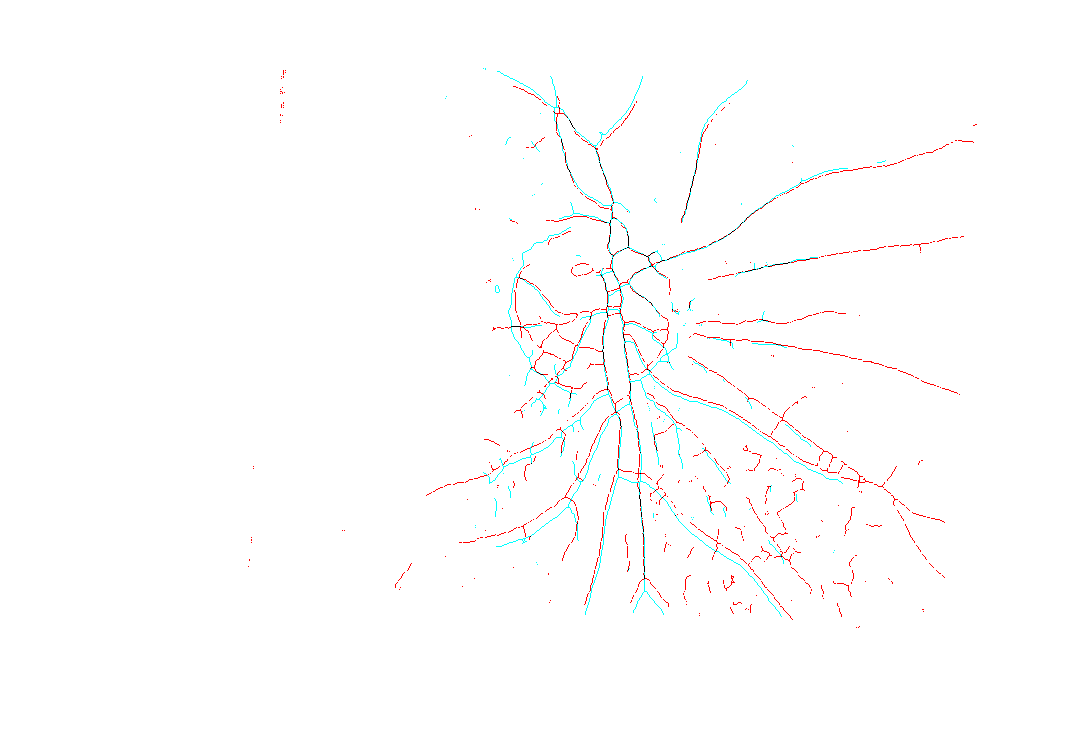
\includegraphics[width=9cm]{cycle1.png}}
\hspace{0.1in}
\subfigure[环血管配准]{
\label{fig:2}
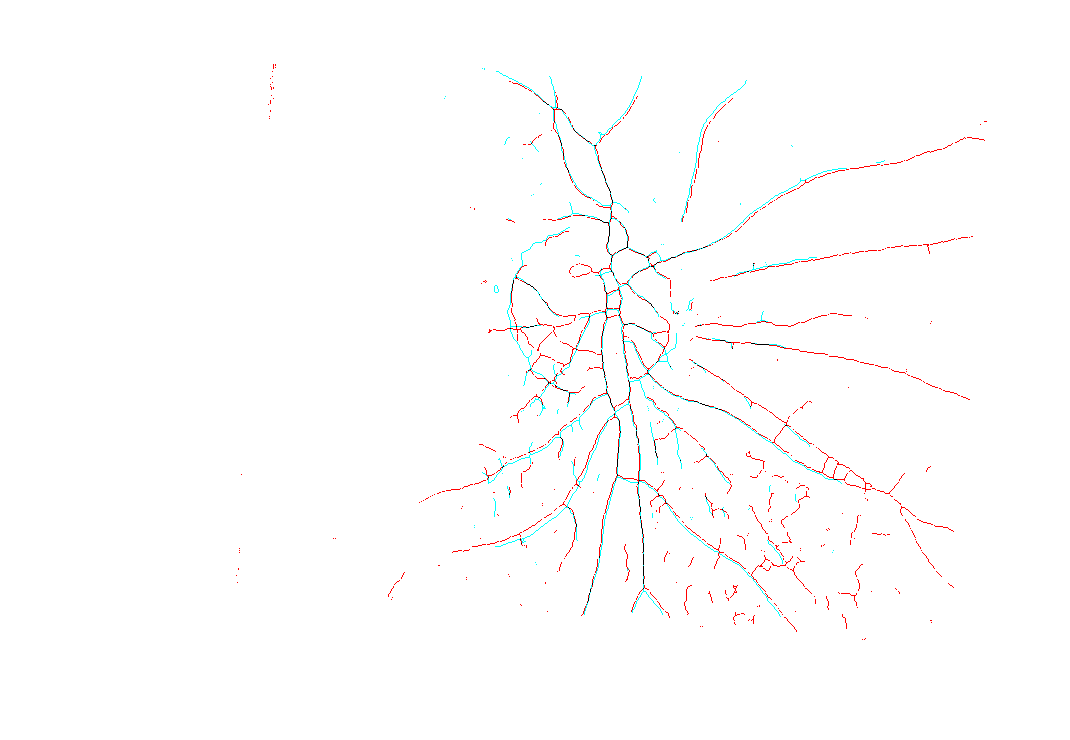
\includegraphics[width=9cm]{cyclevessel1.png}}
\subfigure[局部配准]{
\label{fig:3}
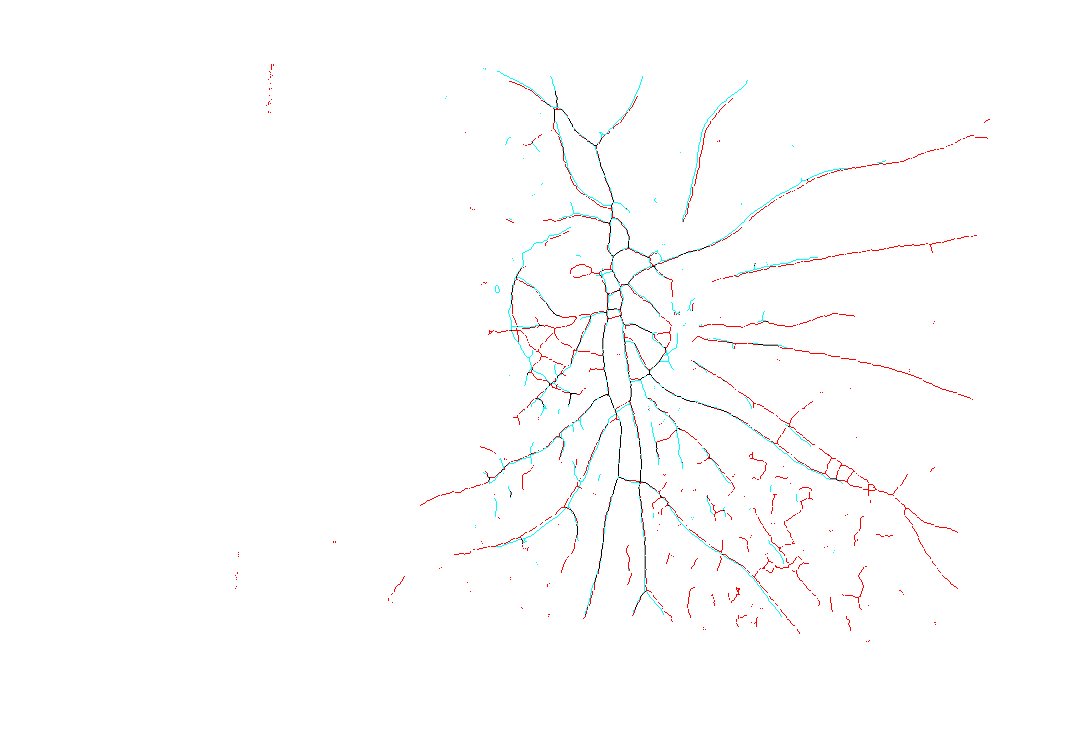
\includegraphics[width=9cm]{local1.png}}
\hspace{0.1in}
\subfigure[二次配准]{
\label{fig:4}
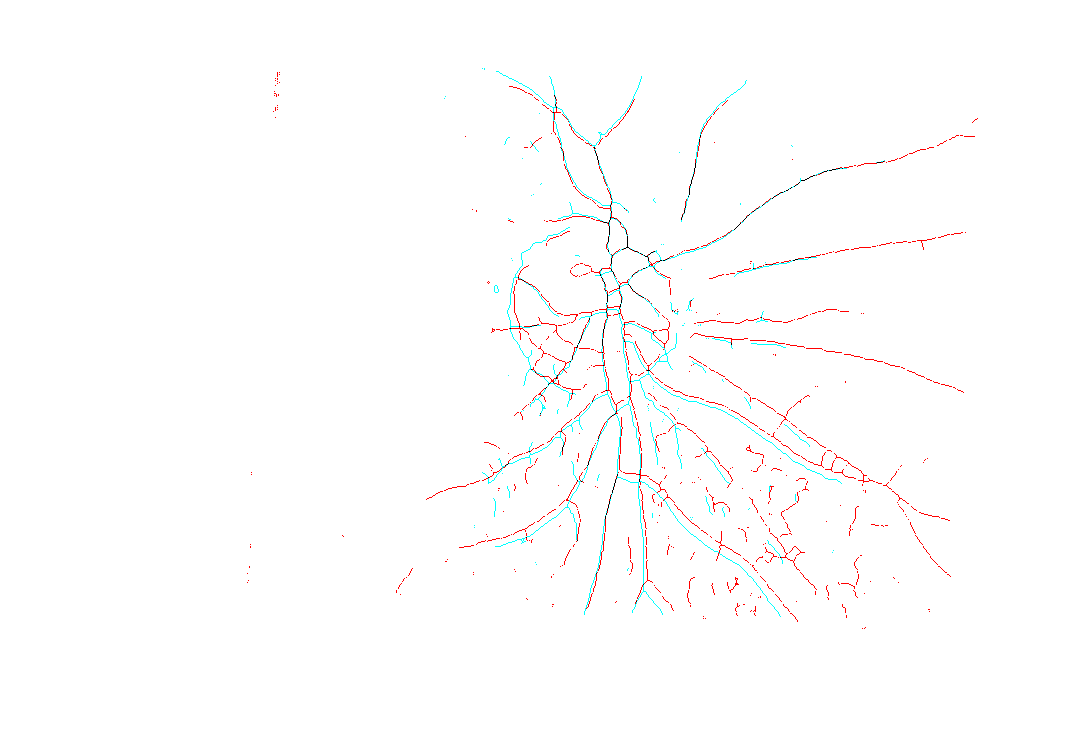
\includegraphics[width=9cm]{twice1.png}}
\caption{varia-1}\label{fig:sub}
\end{figure}

\begin{figure}
\subfigure[只用环结构配准]{
\label{fig:1}
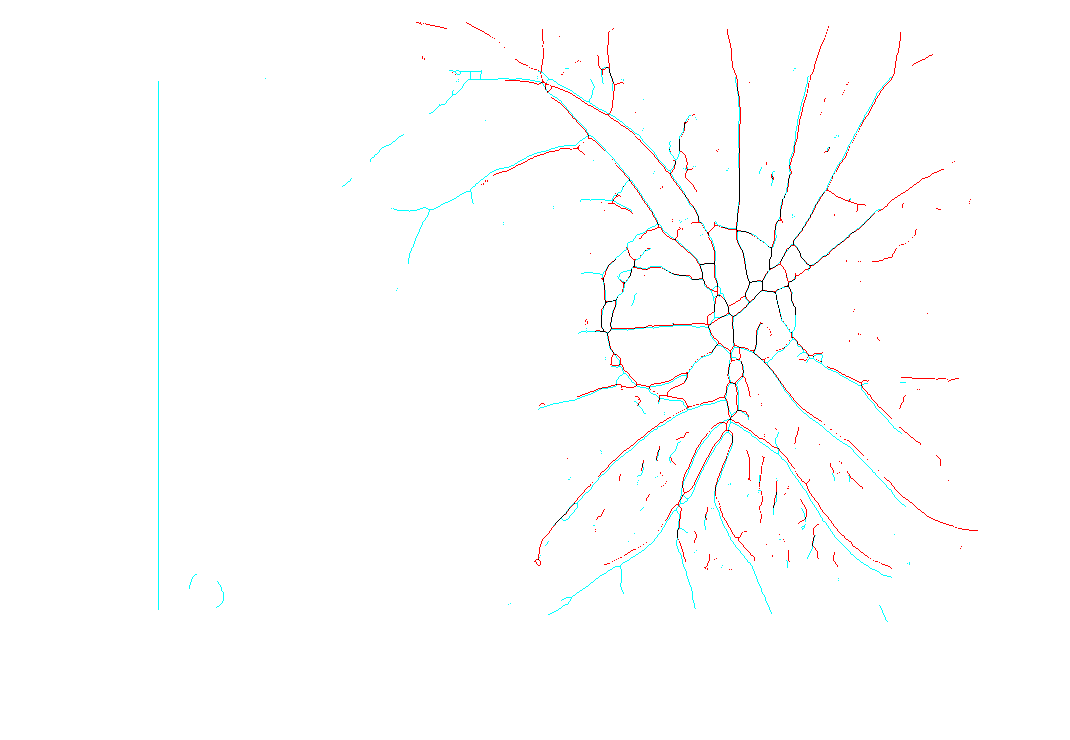
\includegraphics[width=9cm]{cycle2.png}}
\hspace{0.1in}
\subfigure[环血管配准]{
\label{fig:2}
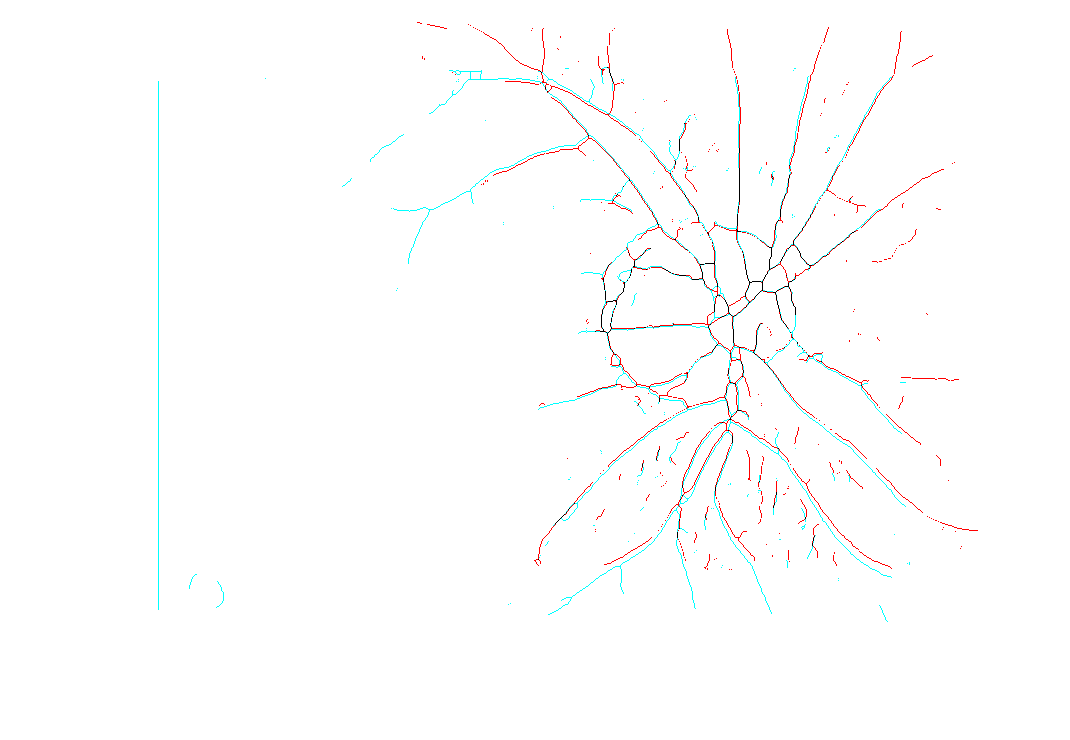
\includegraphics[width=9cm]{cyclevessel2.png}}
\subfigure[局部配准]{
\label{fig:3}
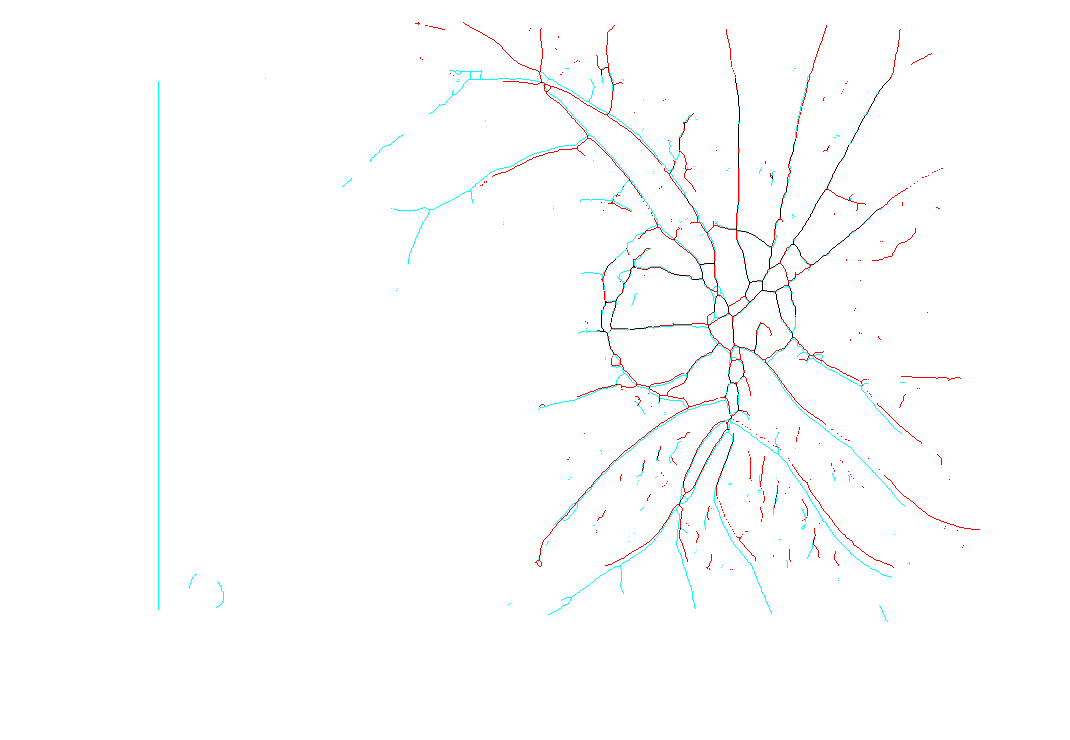
\includegraphics[width=9cm]{local2.png}}
\hspace{0.1in}
\subfigure[二次配准]{
\label{fig:4}
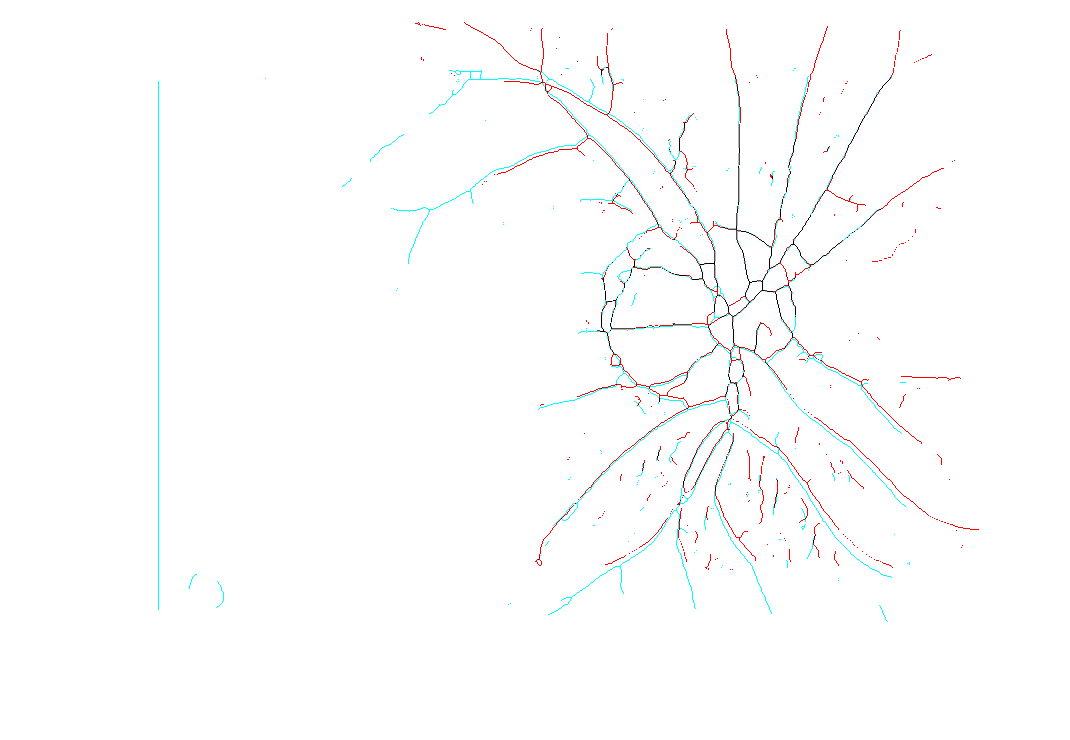
\includegraphics[width=9cm]{twice2.png}}
\caption{varia-2}\label{fig:sub}
\end{figure}

\begin{figure}
%\centering
\subfigure[只用环结构配准]{
\label{fig:1}
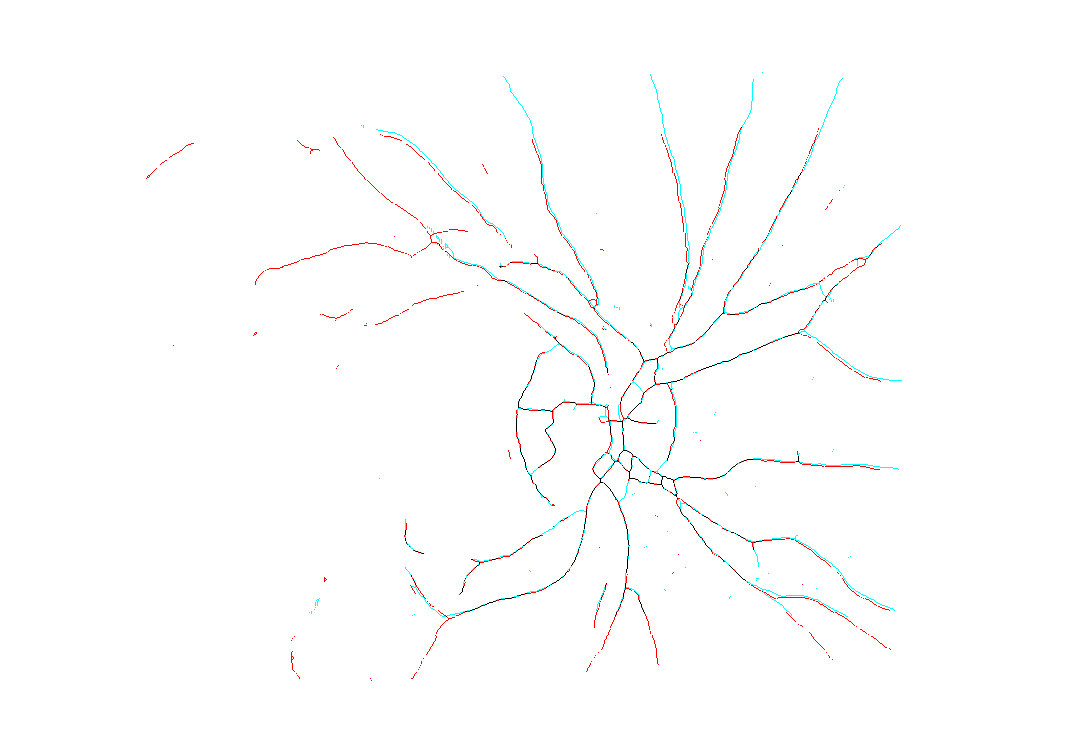
\includegraphics[width=9cm]{cycle3.png}}
\hspace{0.1in}
\subfigure[环血管配准]{
\label{fig:2}
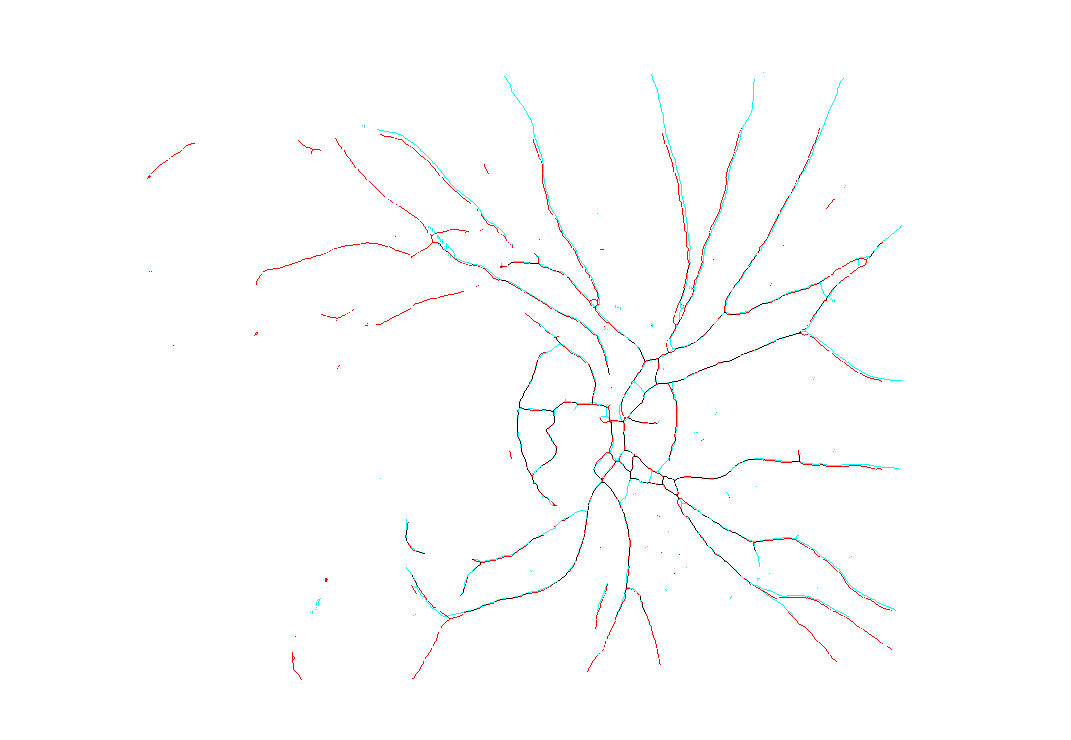
\includegraphics[width=9cm]{cyclevessel3.png}}
\subfigure[局部配准]{
\label{fig:3}
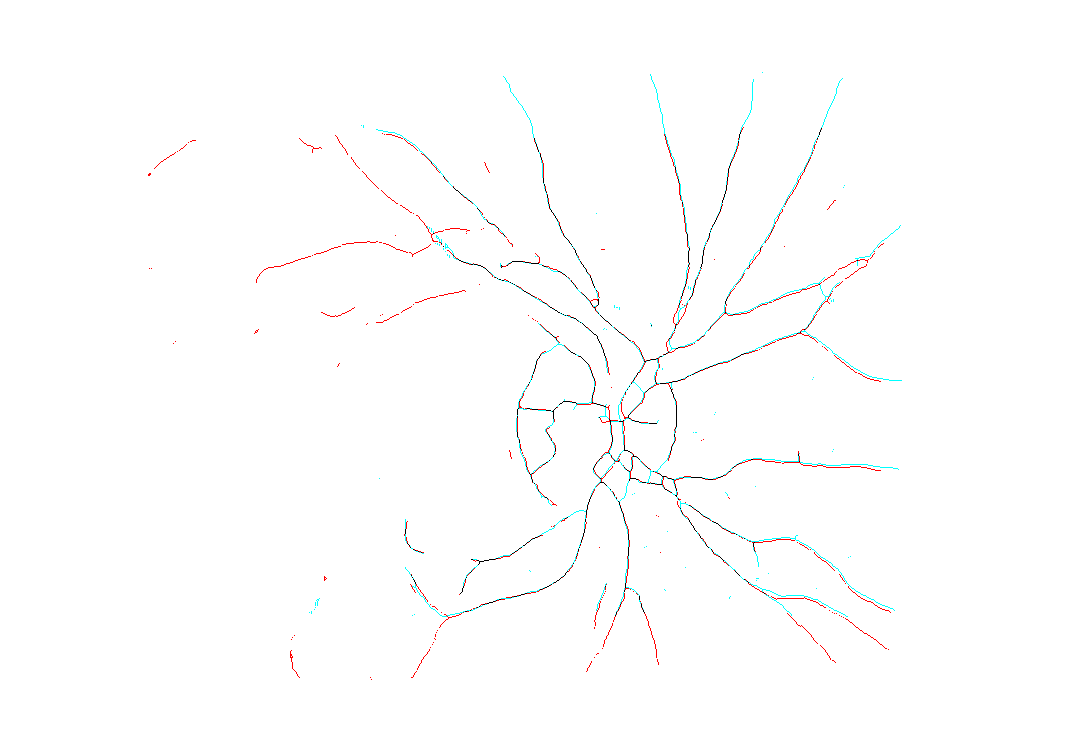
\includegraphics[width=9cm]{local3.png}}
\hspace{0.1in}
\subfigure[二次配准]{
\label{fig:4}
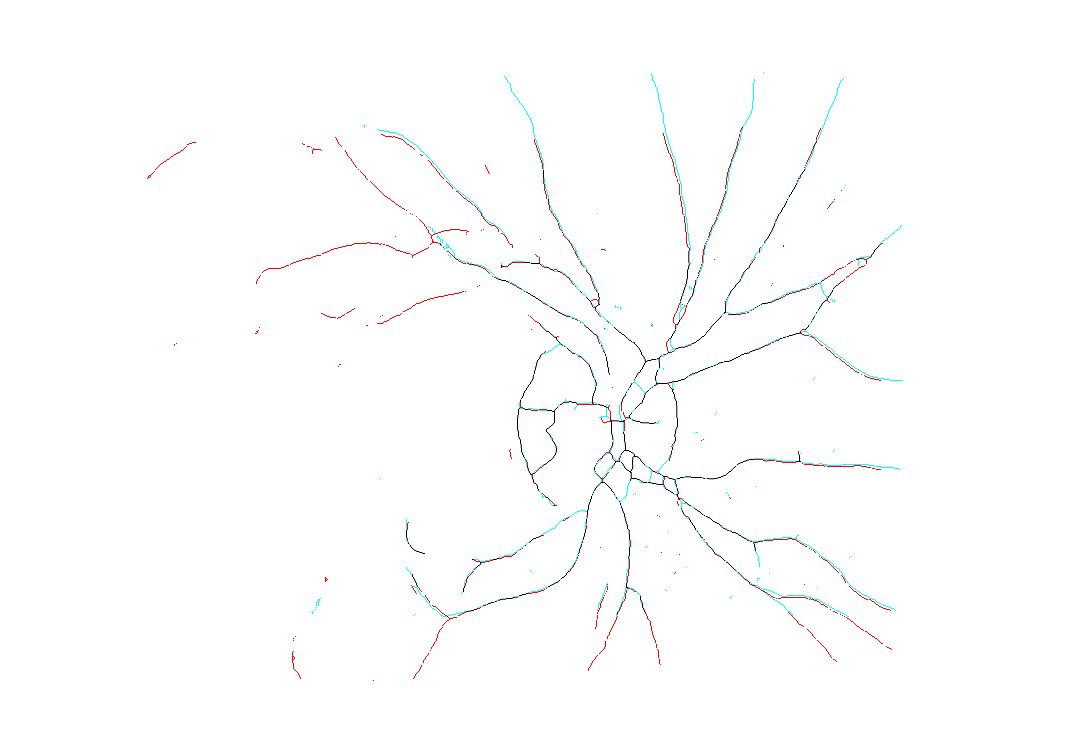
\includegraphics[width=9cm]{twice3.png}}
\caption{varia-3}\label{fig:sub}
\end{figure}

\begin{figure}
%\centering
\subfigure[只用环结构配准]{
\label{fig:1}
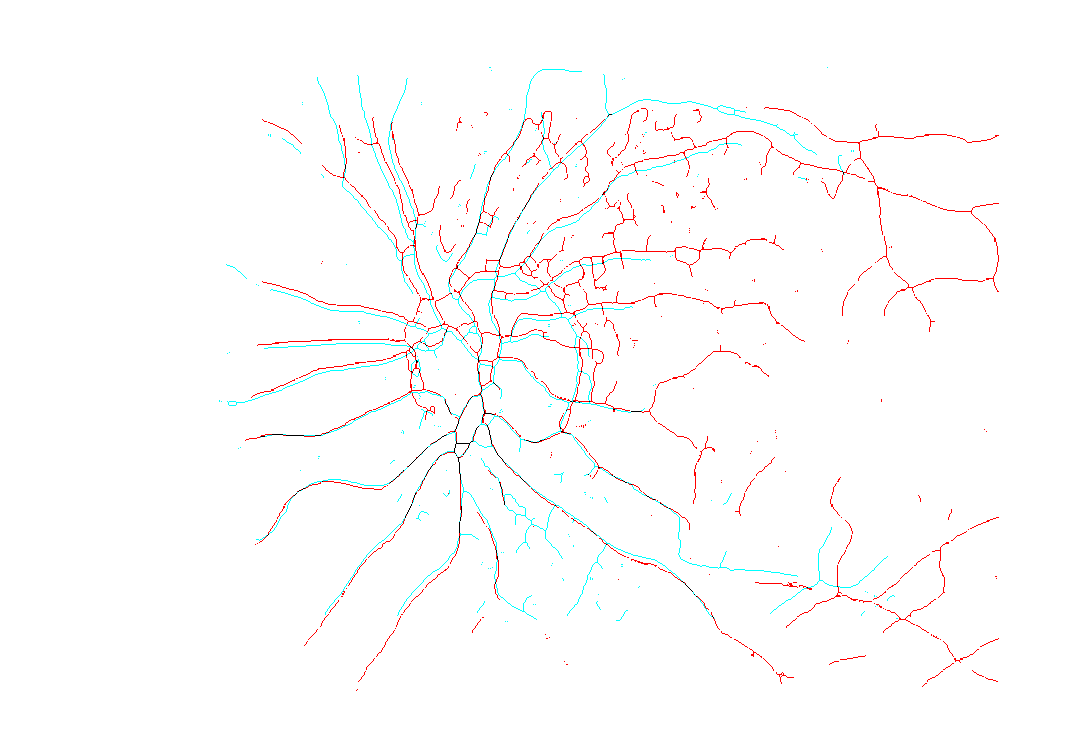
\includegraphics[width=9cm]{cycle5.png}}
\hspace{0.1in}
\subfigure[环血管配准]{
\label{fig:2}
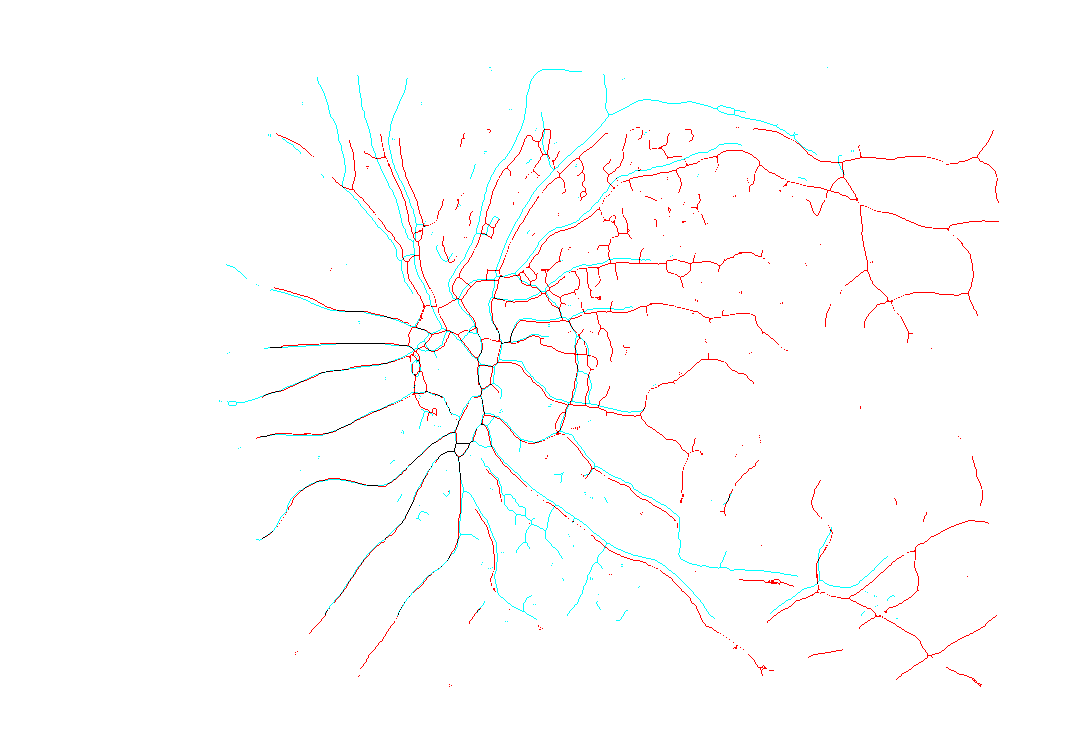
\includegraphics[width=9cm]{cyclevessel5.png}}
\subfigure[局部配准]{
\label{fig:3}
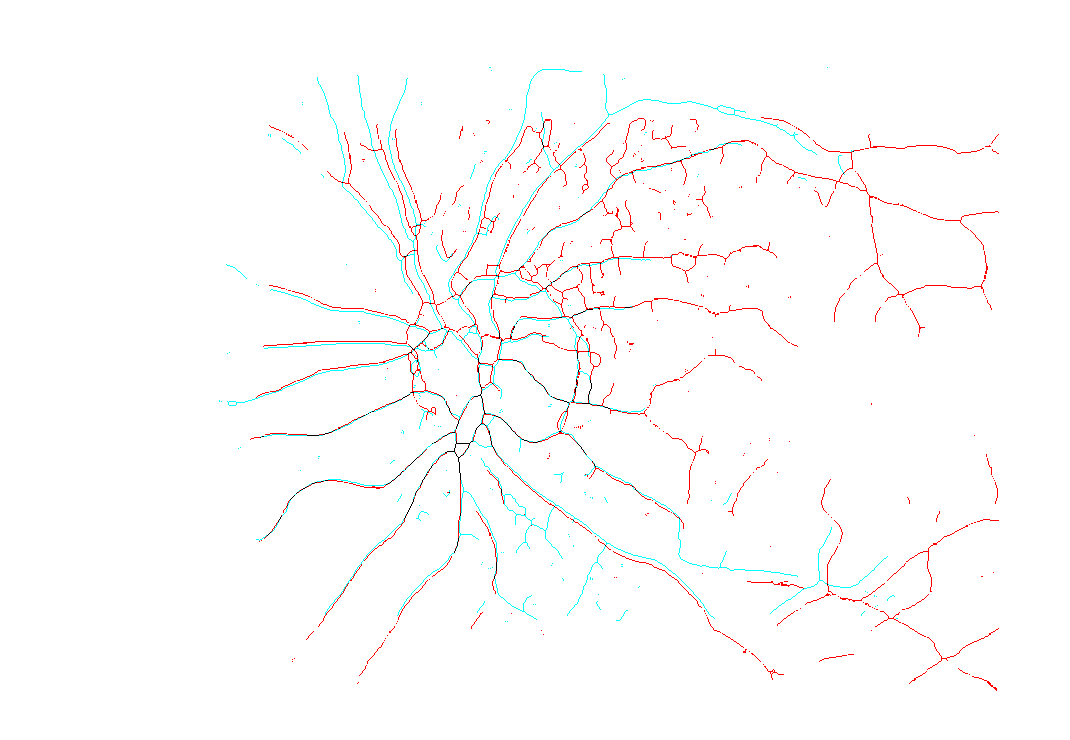
\includegraphics[width=9cm]{local5.png}}
\hspace{0.1in}
\subfigure[二次配准]{
\label{fig:4}
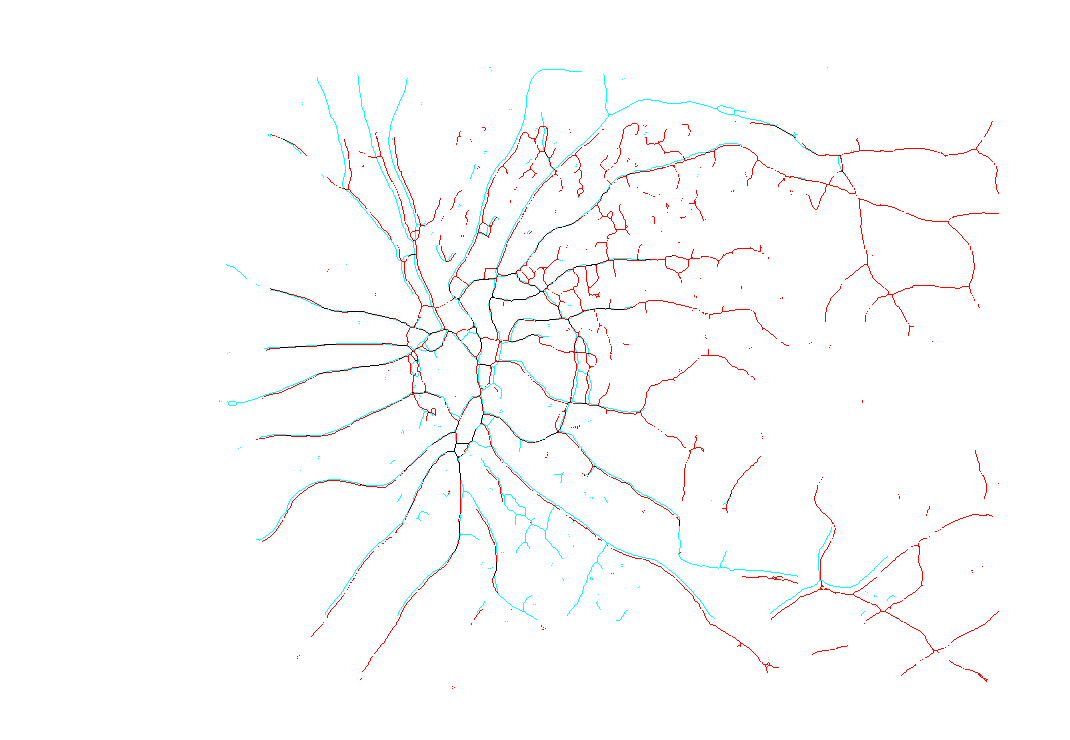
\includegraphics[width=9cm]{twice5.png}}
\caption{varia-5}\label{fig:sub}
\end{figure}

\begin{figure}
%\centering
\subfigure[只用环结构配准]{
\label{fig:1}
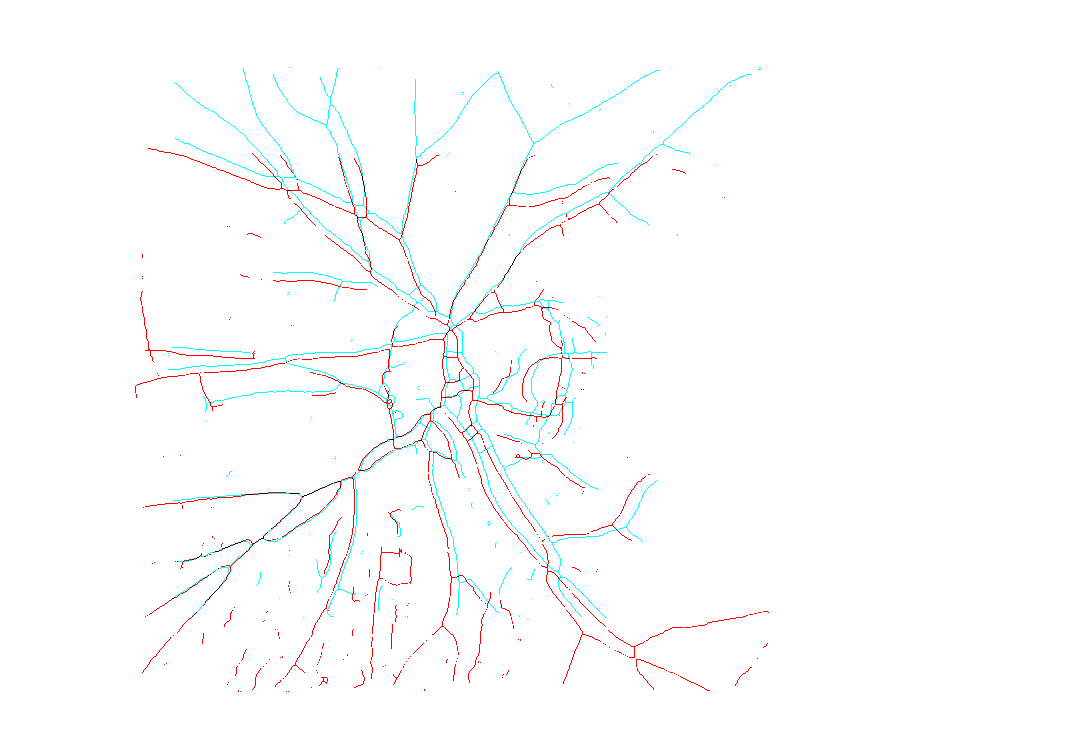
\includegraphics[width=9cm]{cycle6.png}}
\hspace{0.1in}
\subfigure[环血管配准]{
\label{fig:2}
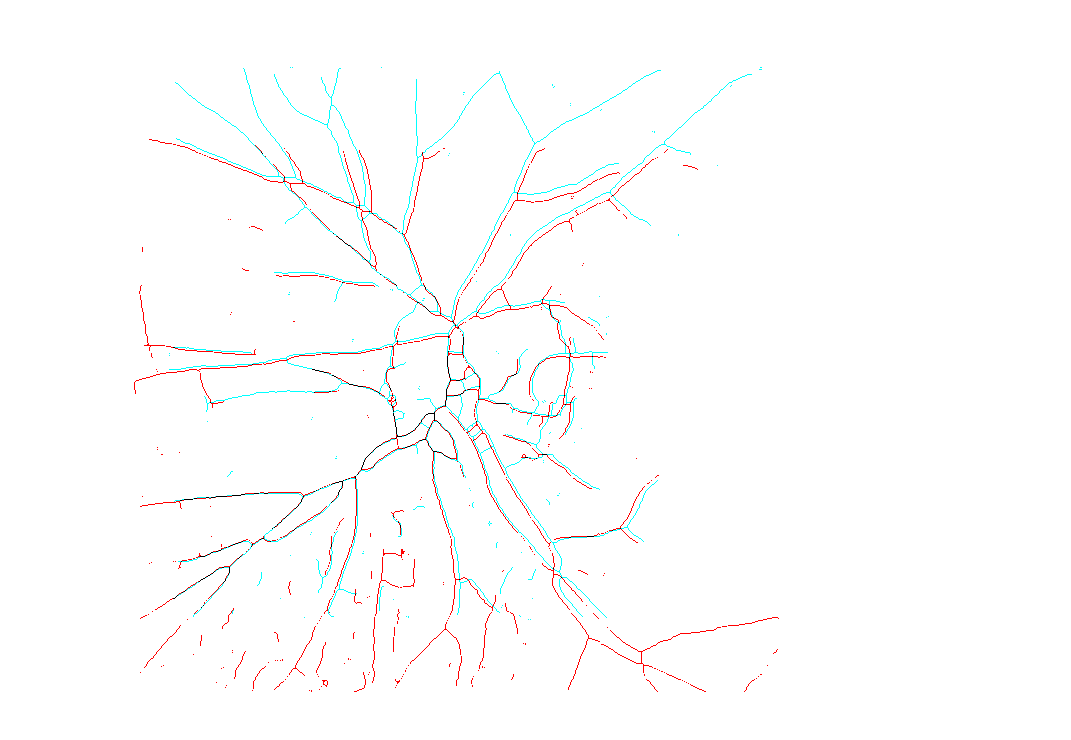
\includegraphics[width=9cm]{cyclevessel6.png}}
\subfigure[局部配准]{
\label{fig:3}
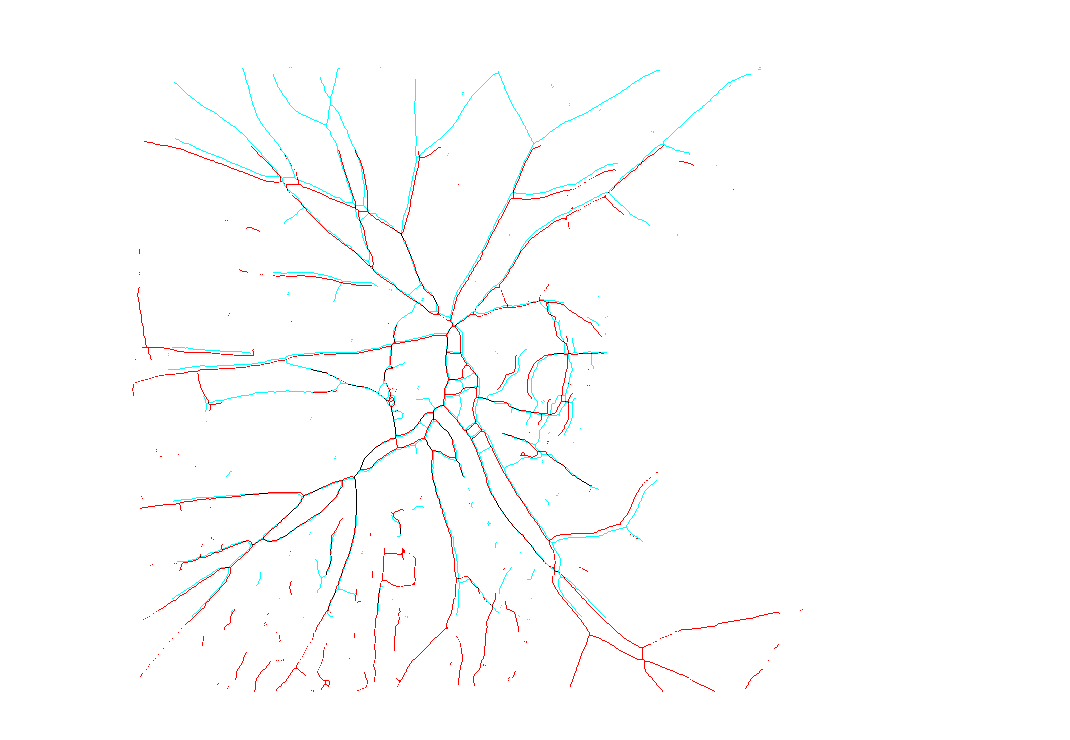
\includegraphics[width=9cm]{local6.png}}
\hspace{0.1in}
\subfigure[二次配准]{
\label{fig:4}
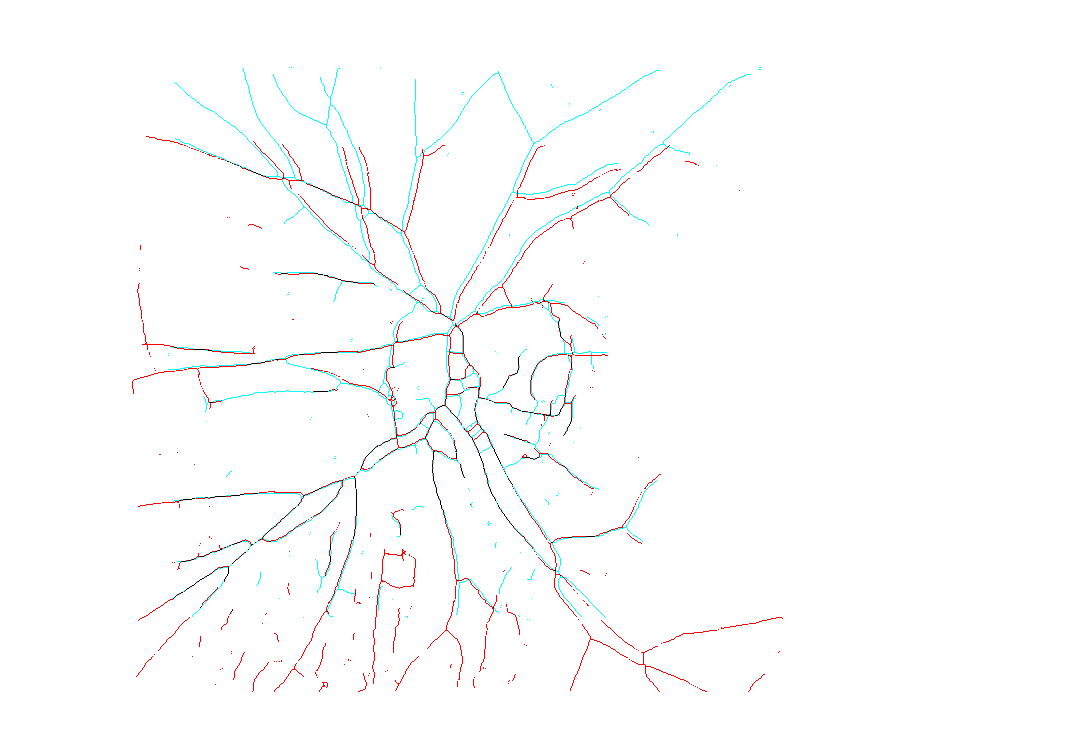
\includegraphics[width=9cm]{twice6.png}}
\caption{varia-6}\label{fig:sub}
\end{figure}

\begin{figure}
%\centering
\subfigure[只用环结构配准]{
\label{fig:1}
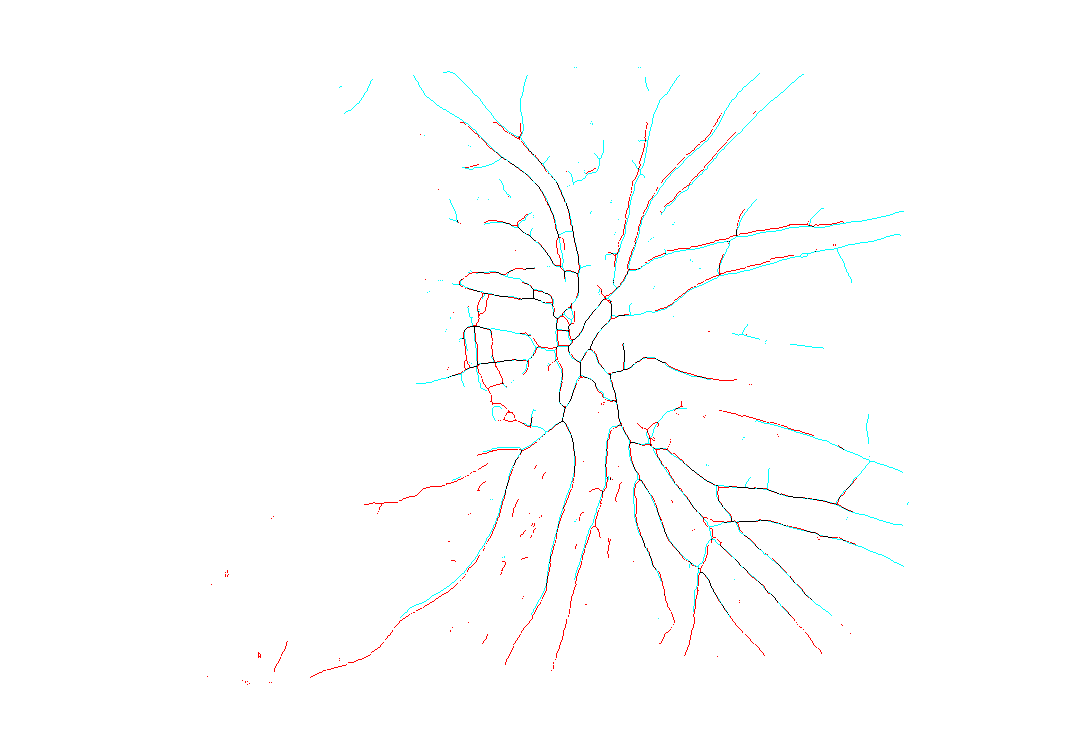
\includegraphics[width=9cm]{cycle7.png}}
\hspace{0.1in}
\subfigure[环血管配准]{
\label{fig:2}
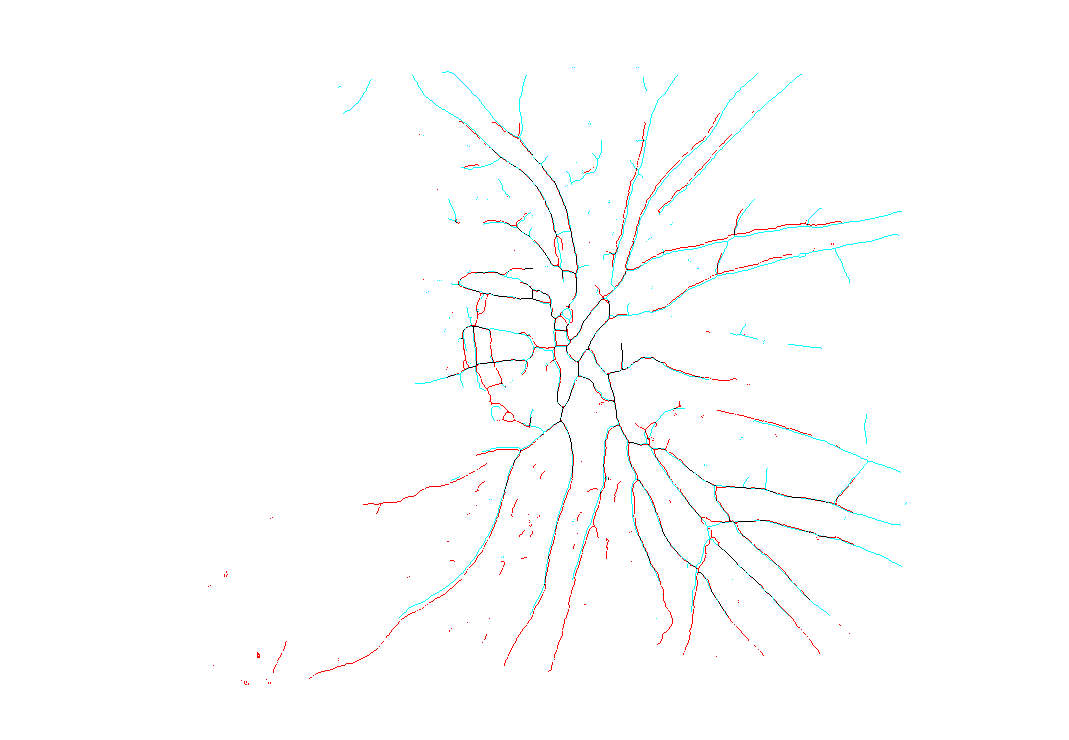
\includegraphics[width=9cm]{cyclevessel7.png}}
\subfigure[局部配准]{
\label{fig:3}
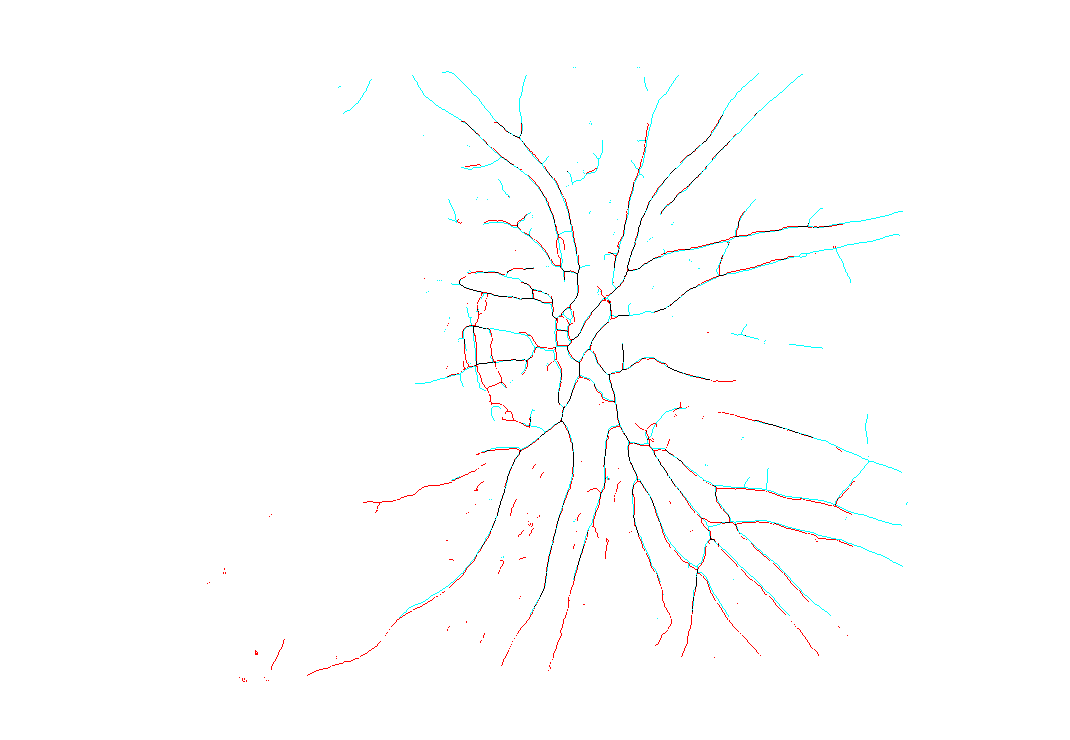
\includegraphics[width=9cm]{local7.png}}
\hspace{0.1in}
\subfigure[二次配准]{
\label{fig:4}
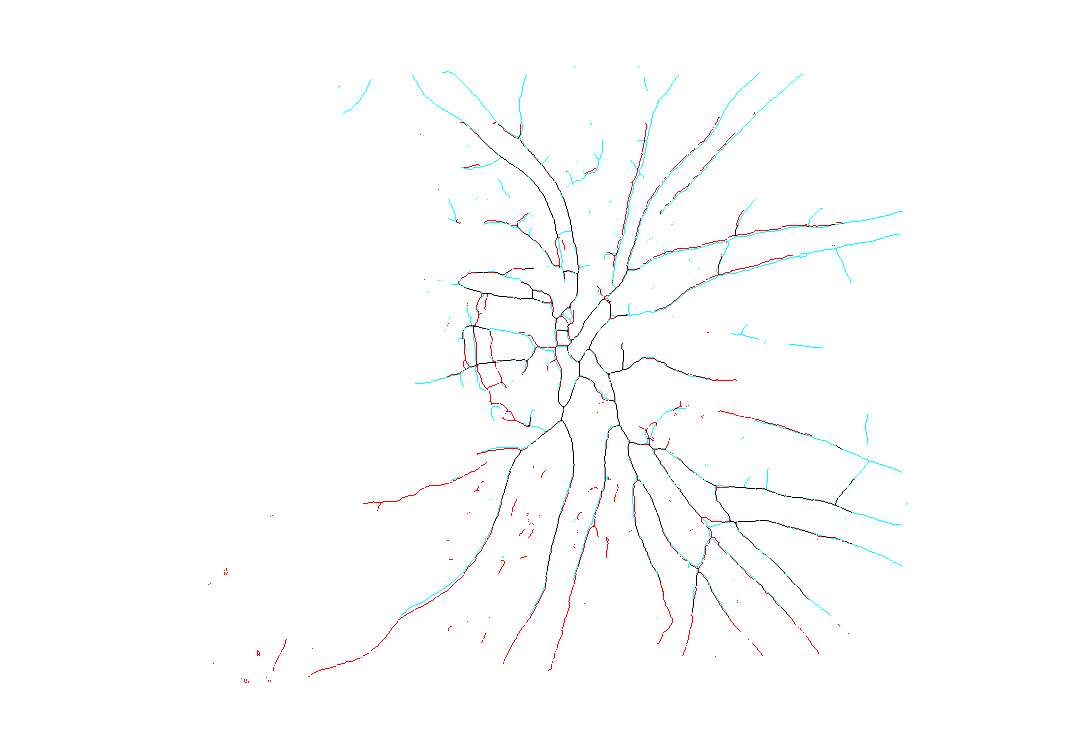
\includegraphics[width=9cm]{twice7.png}}
\caption{varia-7}\label{fig:sub}
\end{figure}

\begin{figure}
%\centering
\subfigure[只用环结构配准]{
\label{fig:1}
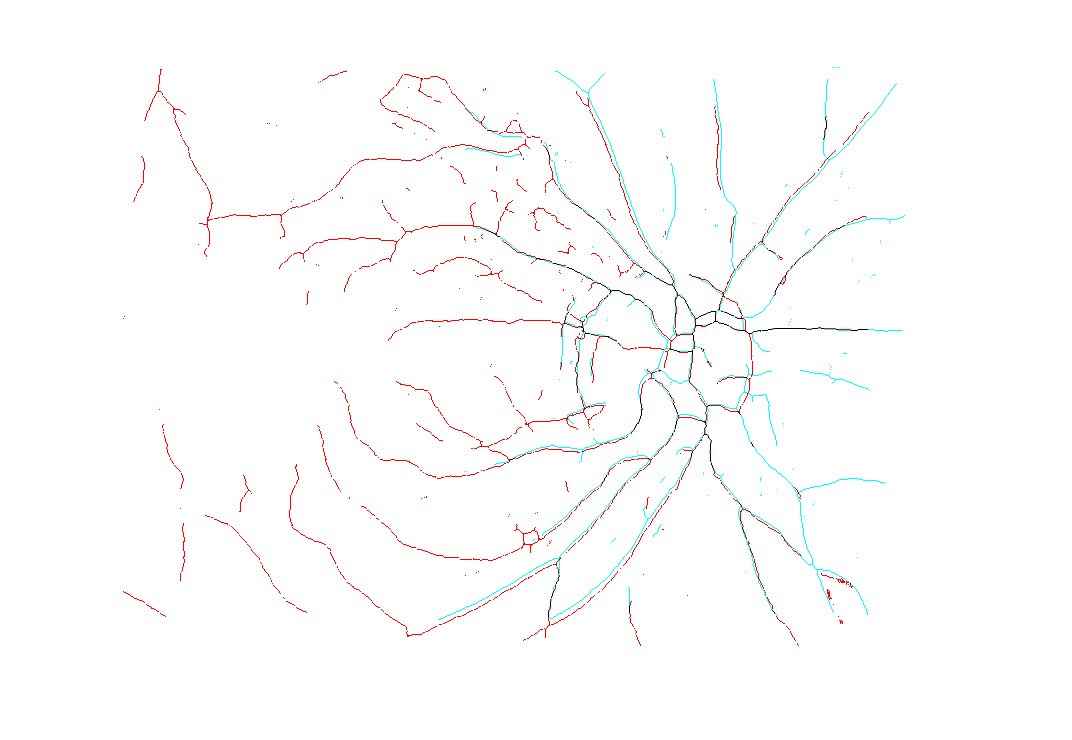
\includegraphics[width=9cm]{cycle8.png}}
\hspace{0.1in}
\subfigure[环血管配准]{
\label{fig:2}
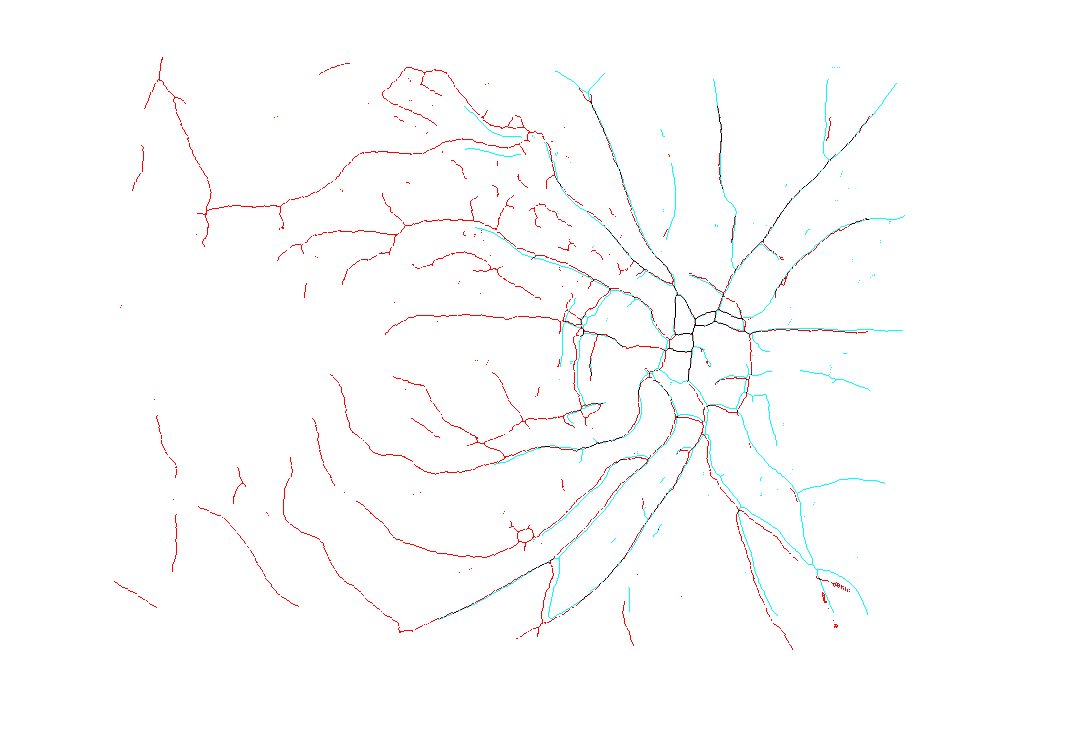
\includegraphics[width=9cm]{cyclevessel8.png}}
\subfigure[局部配准]{
\label{fig:3}
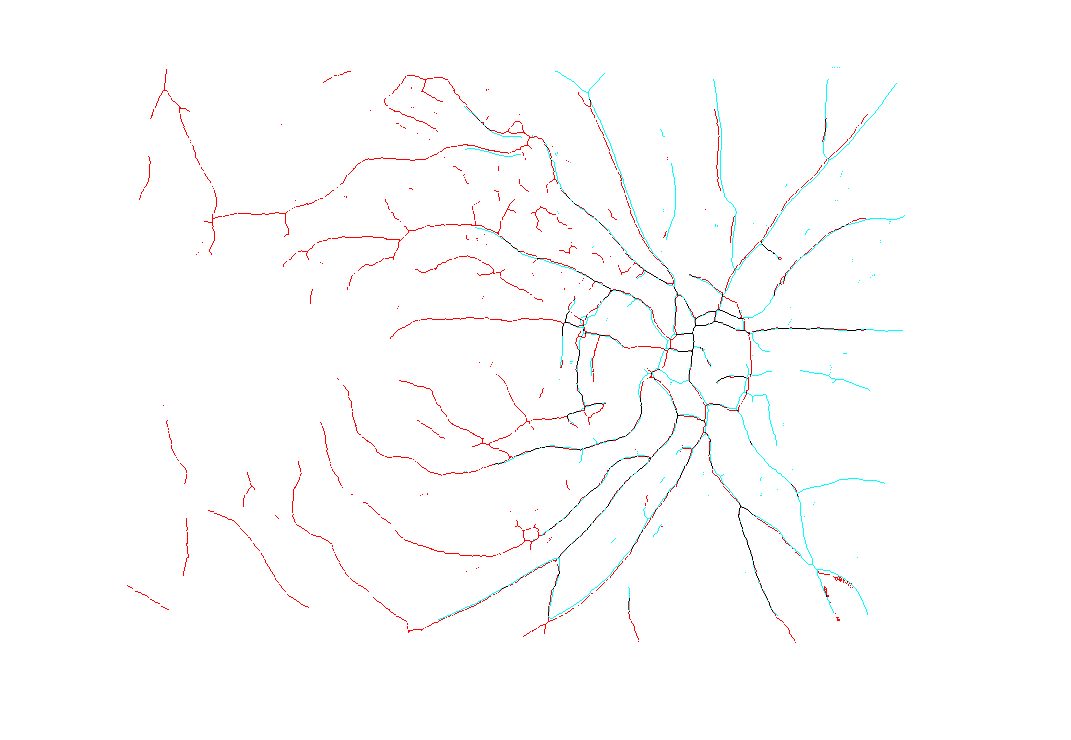
\includegraphics[width=9cm]{local8.png}}
\hspace{0.1in}
\subfigure[二次配准]{
\label{fig:4}
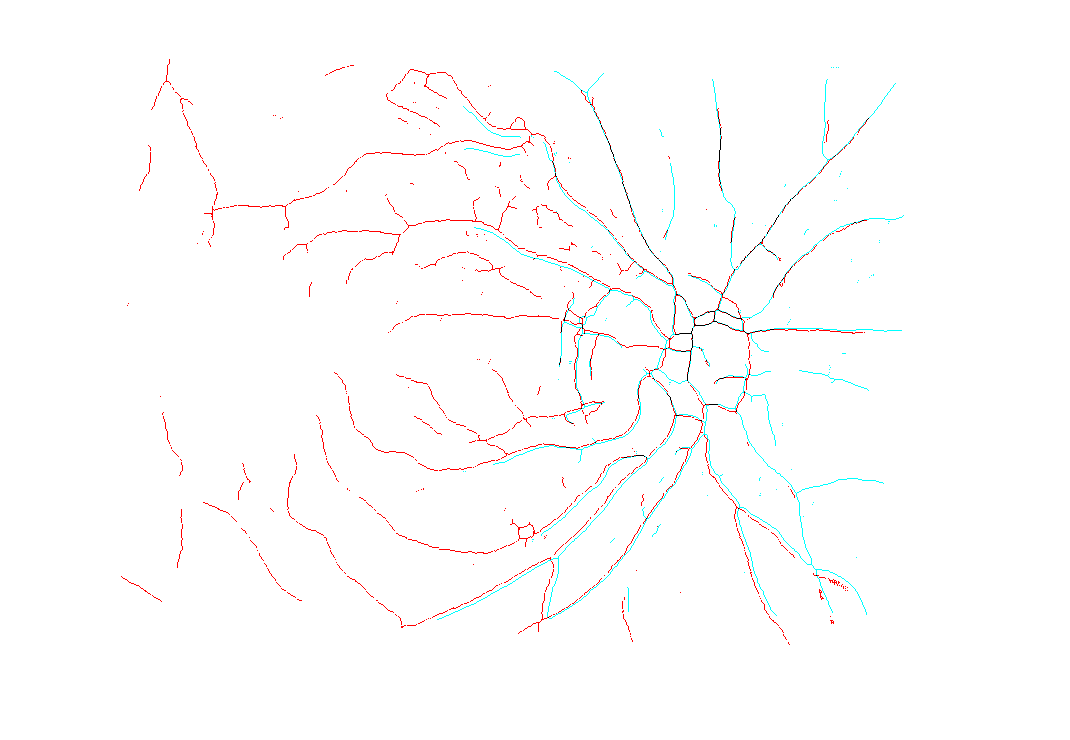
\includegraphics[width=9cm]{twice8.png}}
\caption{varia-8}\label{fig:sub}
\end{figure}

\begin{figure}
%\centering
\subfigure[只用环结构配准]{
\label{fig:1}
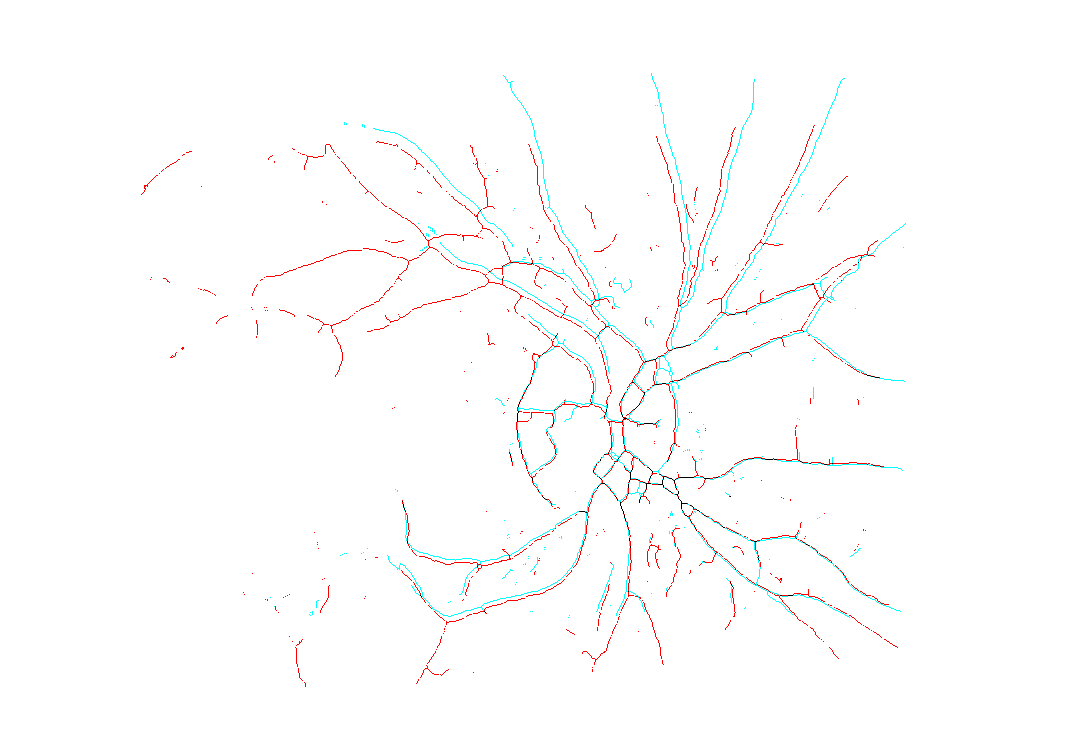
\includegraphics[width=9cm]{cycle9.png}}
\hspace{0.1in}
\subfigure[环血管配准]{
\label{fig:2}
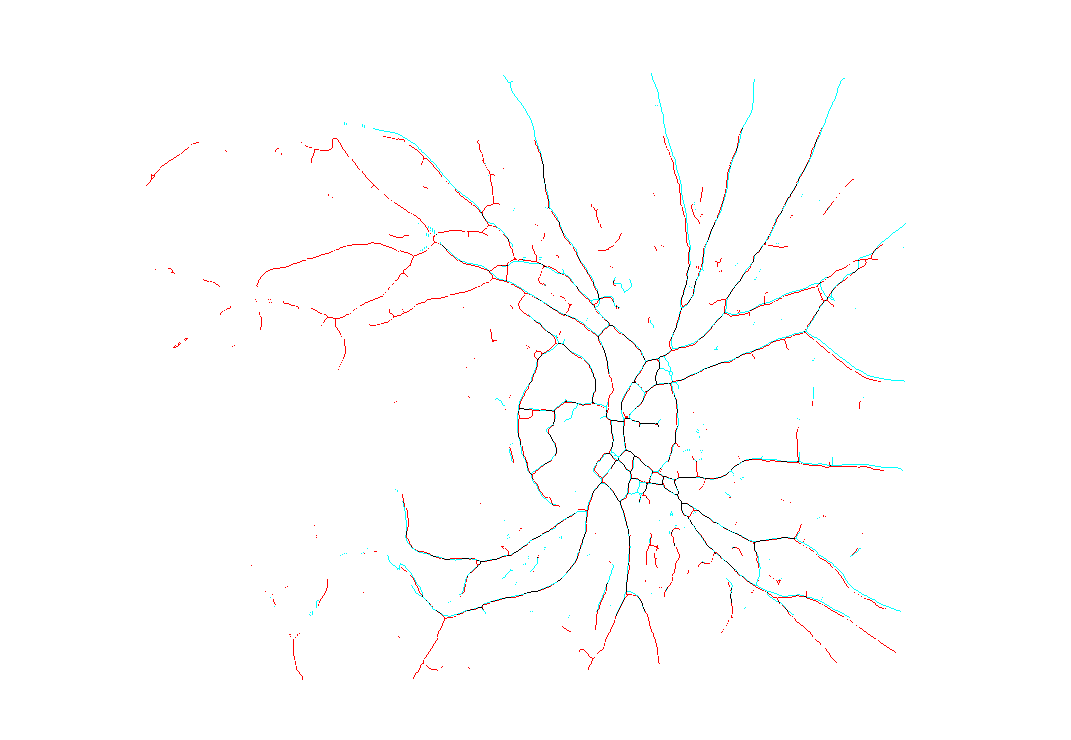
\includegraphics[width=9cm]{cyclevessel9.png}}
\subfigure[局部配准]{
\label{fig:3}
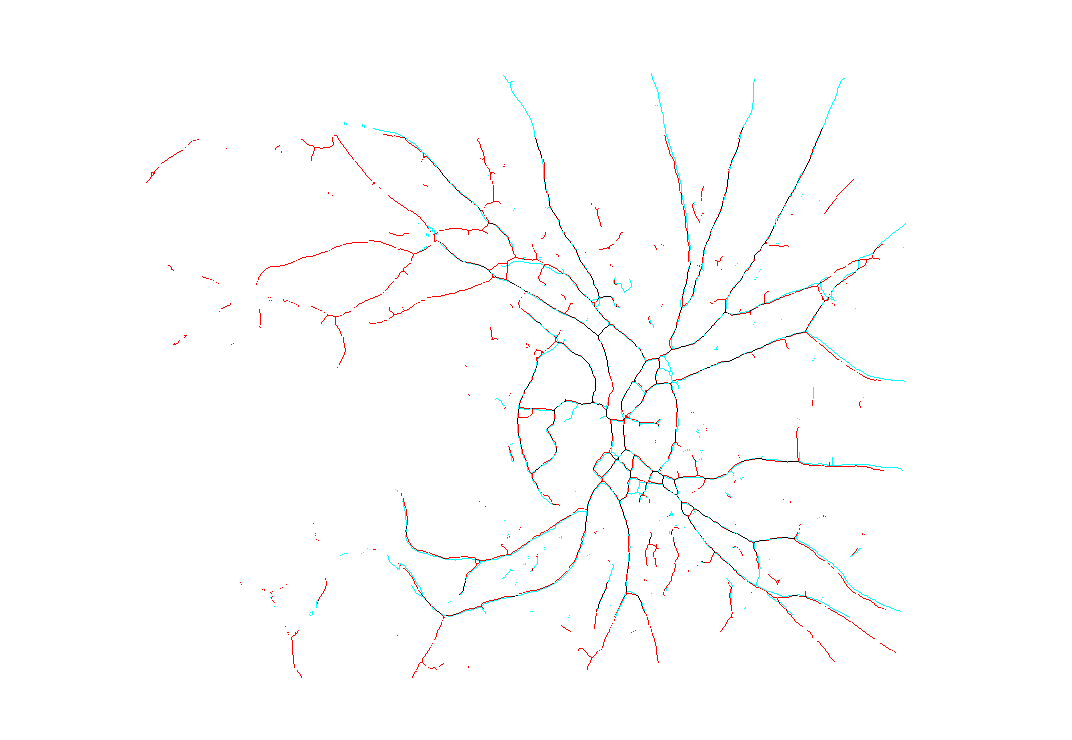
\includegraphics[width=9cm]{local9.png}}
\hspace{0.1in}
\subfigure[二次配准]{
\label{fig:4}
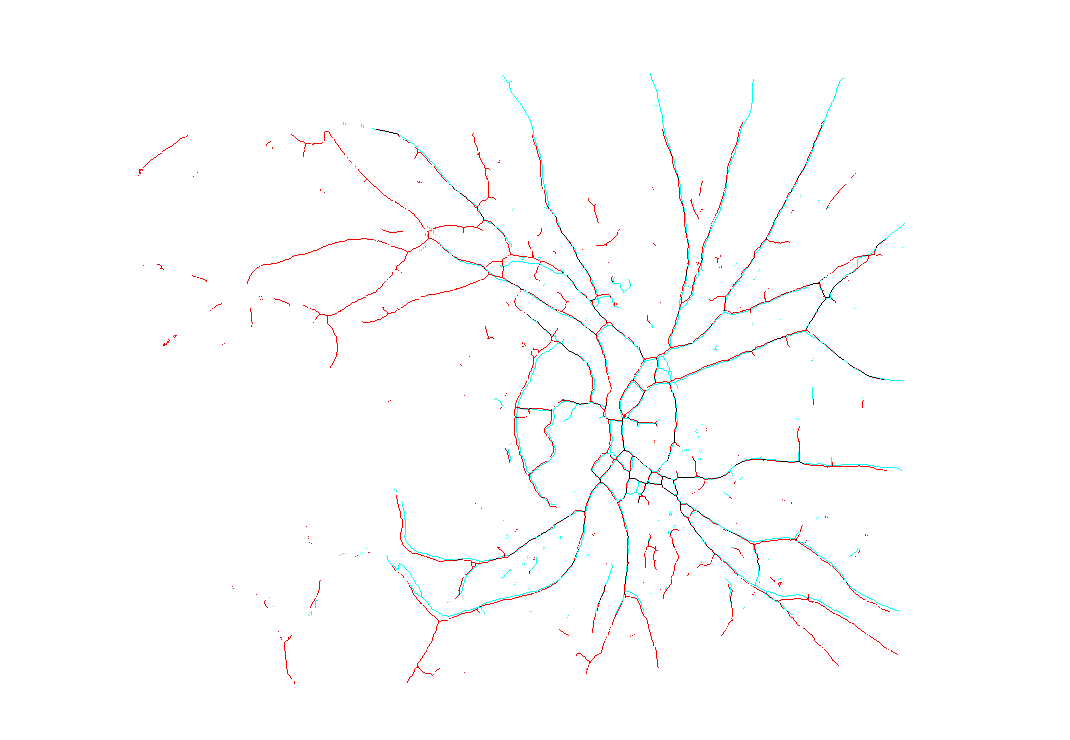
\includegraphics[width=9cm]{twice9.png}}
\caption{varia-9}\label{fig:sub}
\end{figure}

\begin{figure}
%\centering
\subfigure[只用环结构配准]{
\label{fig:1}
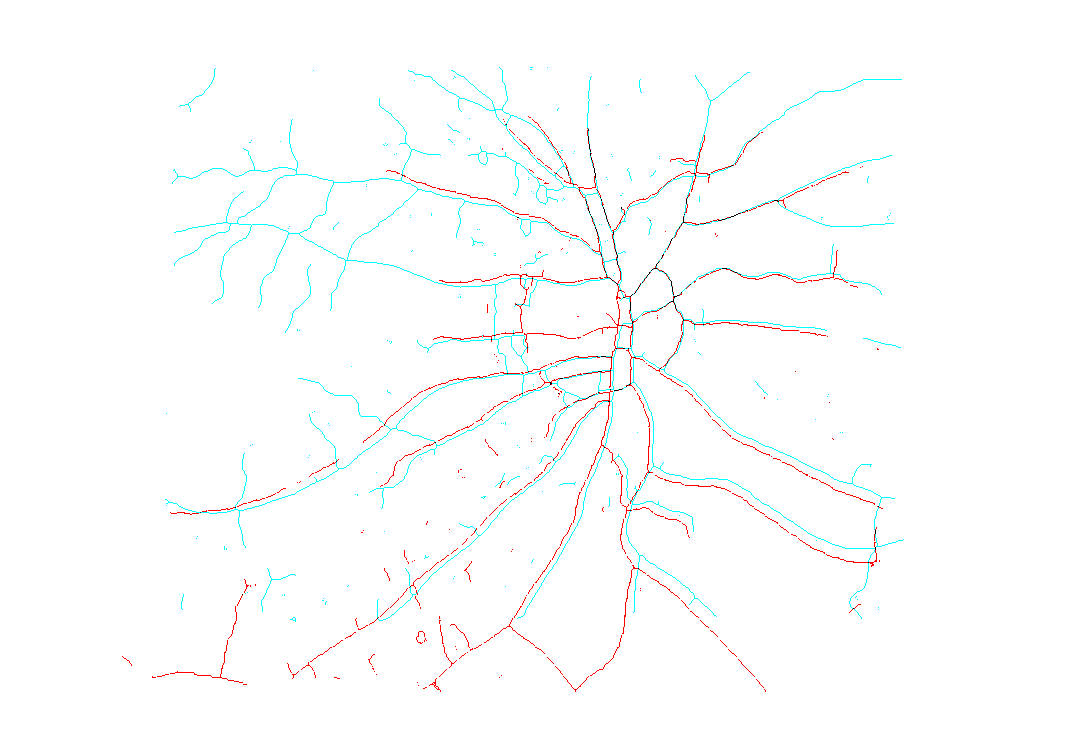
\includegraphics[width=9cm]{cycle10.png}}
\hspace{0.1in}
\subfigure[环血管配准]{
\label{fig:2}
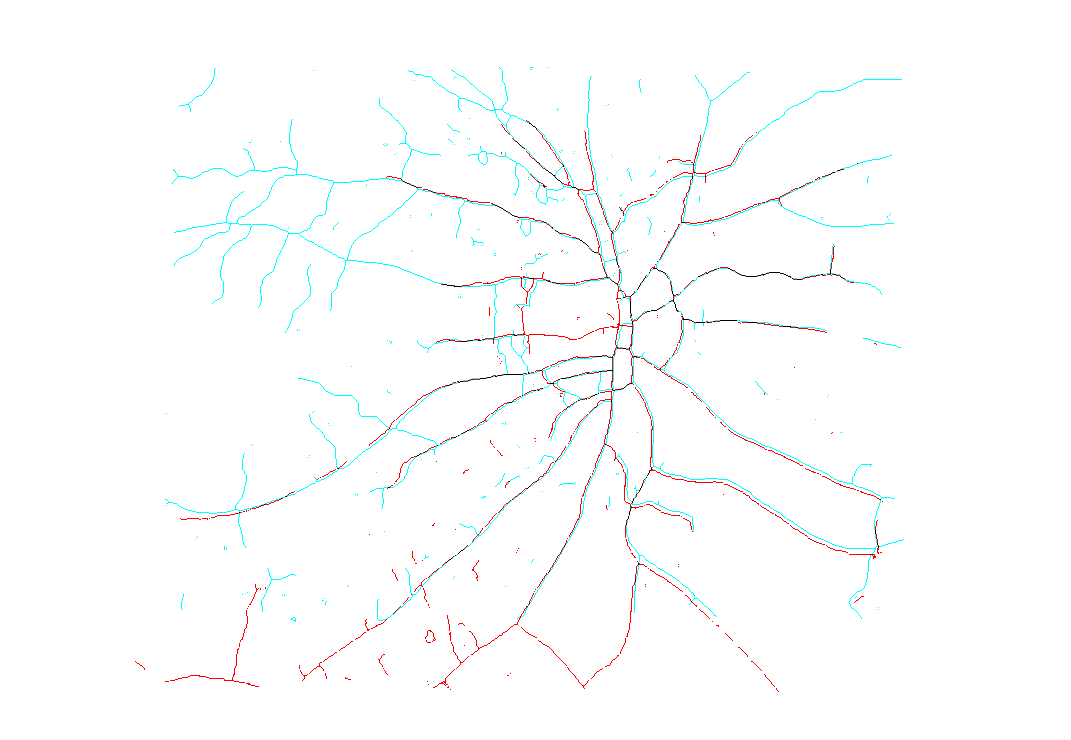
\includegraphics[width=9cm]{cyclevessel10.png}}
\subfigure[局部配准]{
\label{fig:3}
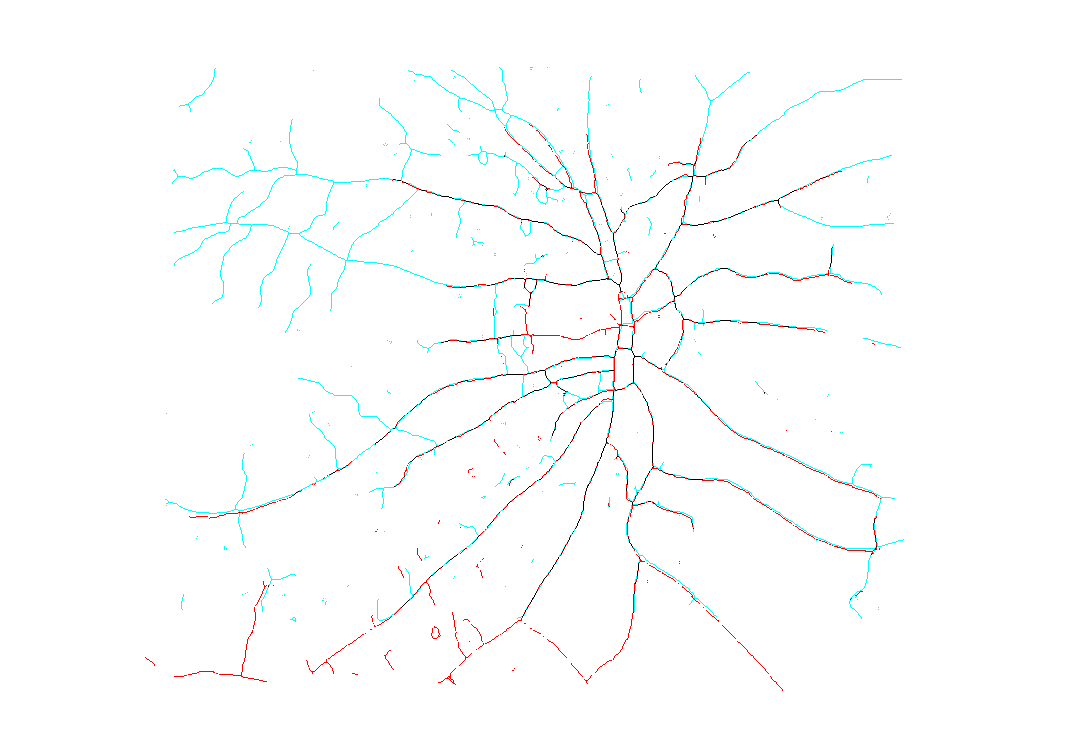
\includegraphics[width=9cm]{local10.png}}
\hspace{0.1in}
\subfigure[二次配准]{
\label{fig:4}
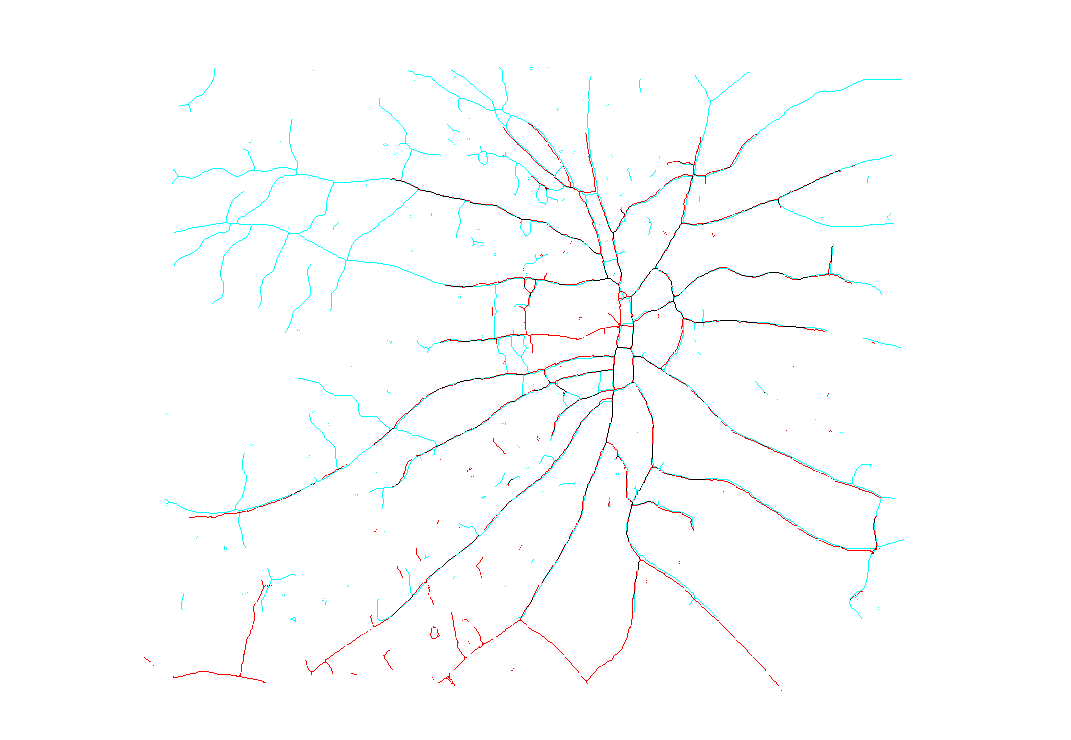
\includegraphics[width=9cm]{twice10.png}}
\caption{varia-10}\label{fig:sub}
\end{figure}

\begin{figure}
%\centering
\subfigure[只用环结构配准]{
\label{fig:1}
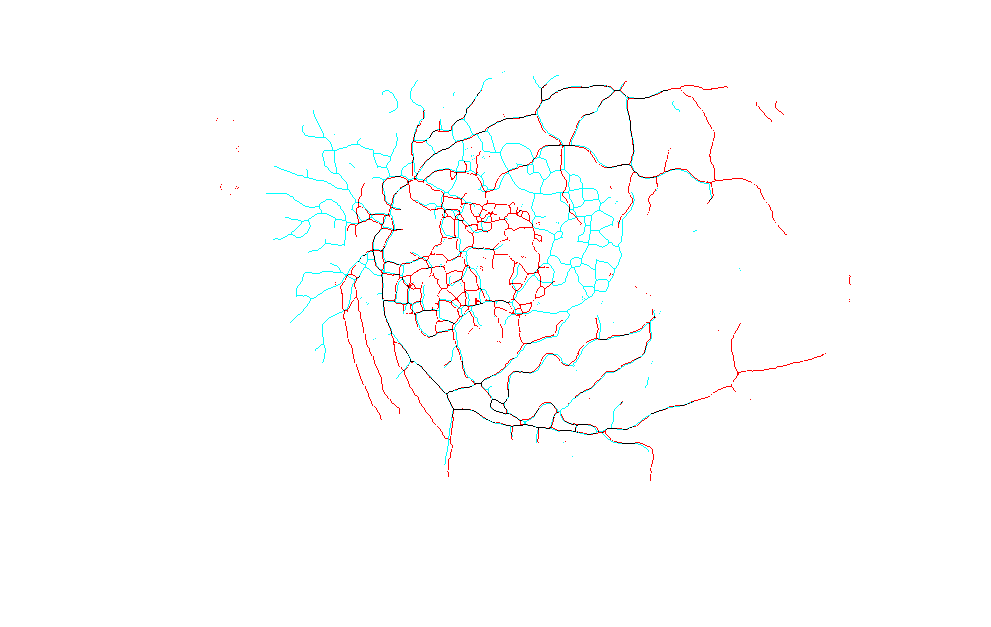
\includegraphics[width=9cm]{cycle11.png}}
\hspace{0.1in}
\subfigure[环血管配准]{
\label{fig:2}
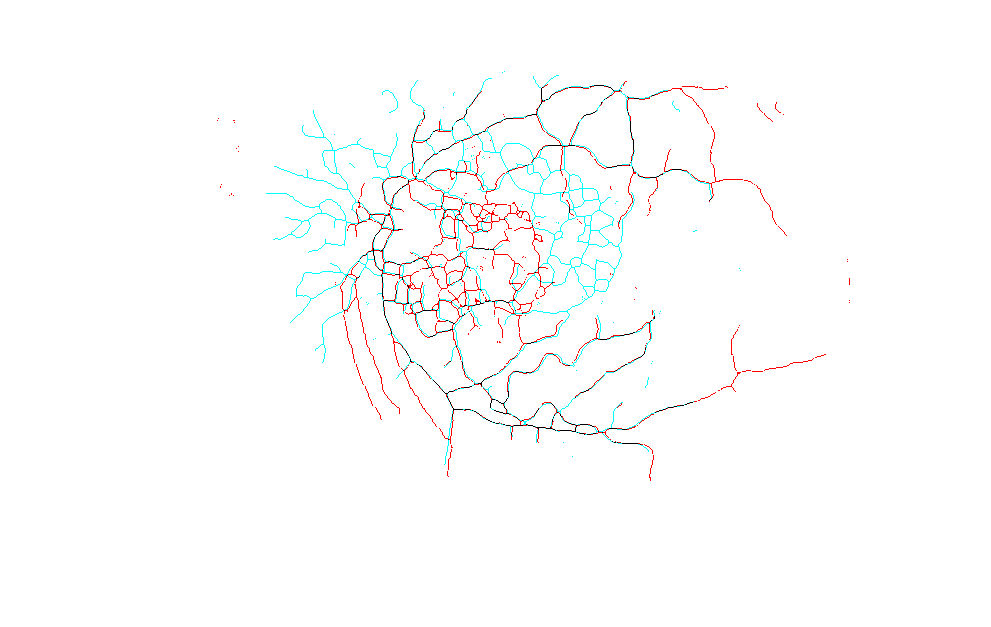
\includegraphics[width=9cm]{cyclevessel11.png}}
\subfigure[局部配准]{
\label{fig:3}
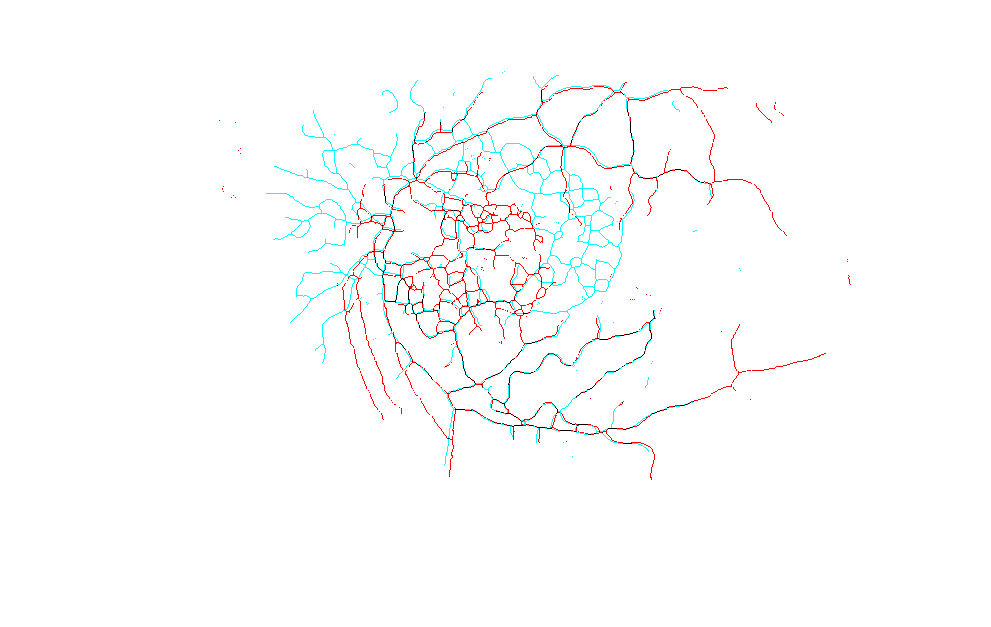
\includegraphics[width=9cm]{local11.png}}
\hspace{0.1in}
\subfigure[二次配准]{
\label{fig:4}
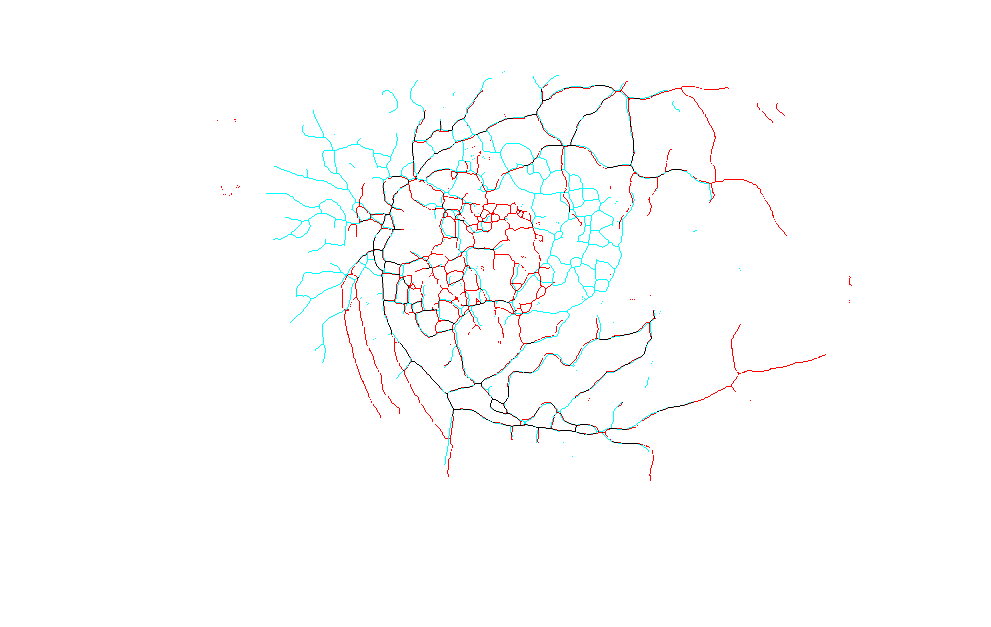
\includegraphics[width=9cm]{twice11.png}}
\caption{其他}\label{fig:sub}
\end{figure}

可知各组实验结果如下:\\
1.局部配准结果>(代表优于)环血管配准结果>只用环结构配准结果,但二次配准的结果比两种方法都差,稍好于只用环的结果。\\
2.环血管配准、局部配准及二次配准效果一般,对只用环的结构改善不大。\\
3.环血管配准、局部配准及二次配准结果略优于只用环结构的配准。\\
5.二次配准结果略优于局部配准>环血管配准结果>只用环结构结果的配准。\\
6.二次配准结果略优于局部配准>环血管配准结果>只用环结构结果的配准。\\
7.环血管配准相比只用环结构的配准结果没有较明显的改善结果,局部配准与二次配准效果相近,均优于环血管、只用环结构的结果。\\
8.局部配准略优于环血管配准>只用环结构配准结果,但二次配准结果比三种都差。\\
9.局部配准>二次配准略优于环血管配准>只用环结构配准结果。\\
10.二次配准略优于局部配准>环血管配准>只用环结构配准结果。\\
11.环血管配准、二次配准结果与只用环结构配准效果相近,略优于局部配准。

\section{实验结果分析}

\noindent 1.在10组实验中,5组二次配准的结果要比只用环结构配准结果好,4组二次配准结果与只用环结构结果差不多或稍好(其中第1组是局部配准、环血管都比只用环结构好),1组二次配准结果比只用环结构差(第8组,但部配准、环血管都比只用环结构好)。\\
2.局部配准、环血管配准均比单用环结构好,其中局部配准效果比较突出,尤其是对局部血管的对齐方面。对整体来说,环血管配准效果比局部配准效果差,且有可能导致最终的二次配准效果不如局部配准效果好\\
3.环血管配准对环所在区域及选取的特征点依赖性比较大,由于分割后的两幅图像上的血管存在一定长度或者形状的差异,经过计算后的对应点可能与实际的对应点相差几个像素,造成对应点的误差;或者由于选取点数较多,某些不太准确的点会影响整体的配准的准确性。对一些图进行一些参数的调节可能会有一定的提高。\\
4.第1、8组出现二次配准比环血管配准、局部配准都差的情况,我们正在分析中。\\


%---------------------------------------------------------------------
\end{document}
